\documentclass[journal]{IEEEtran}
\usepackage{amsmath,amssymb,graphicx,booktabs,multirow,url,xcolor,balance}
\usepackage[caption=false,font=footnotesize]{subfig}
\usepackage[hidelinks]{hyperref}
\graphicspath{{../figures/}{../schematics/}{../layout/png/}}
\newcommand{\mapeIdVgMin}{1.3}
\newcommand{\mapeIdVgMax}{12.1}
\newcommand{\mapeIdVdMin}{3.7}
\newcommand{\mapeIdVdMax}{12.6}
\newcommand{\frosi}{19.39}
\newcommand{\tpdsi}{5.2}
\newcommand{\ecycsi}{2.09}
\newcommand{\pavgsi}{40.6}
\newcommand{\vmsi}{0.49}
\newcommand{\gainsi}{16}
\newcommand{\nmlsi}{0.41}
\newcommand{\nmhsi}{0.44}
\newcommand{\pdpsi}{0.209}
\newcommand{\yfsi}{nan}
\newcommand{\yfuncsi}{nan}
\newcommand{\sigfsi}{nan}
\newcommand{\frosige}{21.39}
\newcommand{\tpdsige}{4.7}
\newcommand{\ecycsige}{2.12}
\newcommand{\pavgsige}{45.4}
\newcommand{\vmsige}{0.49}
\newcommand{\gainsige}{16}
\newcommand{\nmlsige}{0.42}
\newcommand{\nmhsige}{0.43}
\newcommand{\pdpsige}{0.212}
\newcommand{\yfsige}{nan}
\newcommand{\yfuncsige}{nan}
\newcommand{\sigfsige}{nan}
\newcommand{\frotmd}{2.59}
\newcommand{\tpdtmd}{38.7}
\newcommand{\ecyctmd}{0.67}
\newcommand{\pavgtmd}{1.7}
\newcommand{\vmtmd}{0.48}
\newcommand{\gaintmd}{12}
\newcommand{\nmltmd}{0.41}
\newcommand{\nmhtmd}{0.45}
\newcommand{\pdptmd}{0.067}
\newcommand{\yftmd}{nan}
\newcommand{\yfunctmd}{nan}
\newcommand{\sigftmd}{nan}
\newcommand{\frocnt}{45.39}
\newcommand{\tpdcnt}{2.2}
\newcommand{\ecyccnt}{0.84}
\newcommand{\pavgcnt}{38.0}
\newcommand{\vmcnt}{0.50}
\newcommand{\gaincnt}{22}
\newcommand{\nmlcnt}{0.42}
\newcommand{\nmhcnt}{0.41}
\newcommand{\pdpcnt}{0.084}
\newcommand{\yfcnt}{nan}
\newcommand{\yfunccnt}{nan}
\newcommand{\sigfcnt}{nan}
\newcommand{\frogan}{1.69}
\newcommand{\tpdgan}{59.1}
\newcommand{\ecycgan}{94.17}
\newcommand{\pavggan}{159.4}
\newcommand{\vmgan}{0.42}
\newcommand{\gaingan}{18}
\newcommand{\nmlgan}{0.25}
\newcommand{\nmhgan}{0.49}
\newcommand{\pdpgan}{9.417}
\newcommand{\yfgan}{nan}
\newcommand{\yfuncgan}{nan}
\newcommand{\sigfgan}{nan}
\newcommand{\tcfgan}{nan}
\newcommand{\fFiveHundredgan}{nan}
\newcommand{\tcfsi}{nan}
\newcommand{\fFiveHundredsi}{nan}
\newcommand{\areainvcfetsi}{8640}
\newcommand{\arearoFivecfetsi}{54000}
\newcommand{\areainvcfetsige}{8640}
\newcommand{\arearoFivecfetsige}{54000}
\newcommand{\areainvcfettmd}{10368}
\newcommand{\arearoFivecfettmd}{64800}
\newcommand{\areainvcfetcnt}{10368}
\newcommand{\arearoFivecfetcnt}{64800}
\newcommand{\areainvcfetgan}{160000}
\newcommand{\arearoFivecfetgan}{1000000}

\newcommand{\ucm}{UCM-CFET}

\begin{document}
\title{A Unified Physics-Based Compact Model and Calibrated Circuit-Validation Flow for Multi-Material CFET Logic: Si, SiGe, MoS$_2$/WSe$_2$, CNT and GaN}

\author{M.~Nisha~Angeline,~\IEEEmembership{Senior Member,~IEEE}%
\thanks{M. Nisha Angeline is with the Department of Electronics and Communication Engineering, Velalar College of Engineering and Technology, Thindal, Erode, Tamil Nadu, India (e-mail: nishavlsidesign@gmail.com).}%
\thanks{Simulation sources, Verilog-A models, Cadence scripts, GDSII layouts and result files are available at the companion repository (branch \texttt{cfet\_multimaterial}).}}

\markboth{IEEE Transactions on Electron Devices}{Nisha Angeline: Multi-material CFET compact model and circuit-validation flow}
\maketitle

\begin{abstract}
Complementary FET (CFET) stacking removes the n/p lateral separation from the standard-cell footprint, but the choice of channel material for the two tiers is still open. We present a unified, physics-based compact model (\ucm) whose single equation core (EKV-type smooth overdrive, velocity-saturation-limited drift--diffusion current with a $\tanh$ drain-voltage interpolation, charge-conserving terminal charges, series resistance and temperature dependence) is extended by material blocks: quantum capacitance and trap-limited ideality for two-dimensional MoS$_2$/WSe$_2$ channels, a Landauer quasi-ballistic branch with a metallic-tube shunt for carbon-nanotube (CNT) arrays, and an electro-thermal node for GaN. Nine device models (Si GAA n/p, SiGe p, MoS$_2$ n, WSe$_2$ p, CNT n/p, GaN n and projected p-GaN) are written once as Verilog-A for Cadence Spectre/ADE, mirrored exactly (within 0.1\%) by an open-source ngspice behavioural library, and calibrated by least squares to literature-anchored reference $I$--$V$ data with \mapeIdVgMin--\mapeIdVgMax\% mean absolute percentage error on $I_D$--$V_G$ and \mapeIdVdMin--\mapeIdVdMax\% on $I_D$--$V_D$ families. The calibrated models drive a common CFET inverter cell with explicit inter-tier coupling capacitance, output parasitic and local-interconnect resistance, 5/7/9-stage ring oscillators (ROs), unified $V_{DD}$ and temperature sweeps, material-specific sensitivity studies and Monte Carlo yield analysis. At nominal supply the 5-stage ROs run at \frosi, \frosige, \frotmd, \frocnt\ and \frogan~GHz for the Si, SiGe, TMD, CNT and GaN platforms with \ecycsi, \ecycsige, \ecyctmd, \ecyccnt\ and \ecycgan~fJ per cycle. A contact-resistance crossover map shows the TMD CFET keeps an iso-frequency energy advantage over Si only below a critical contact resistance; the CNT platform is limited by metallic-tube leakage above $10^{-3}$ purity defects; the GaN platform shows a frequency temperature coefficient of \tcfgan~ppm/K between 300 and 500~K. The outcome is a material-selection map rather than a single winner, together with conceptual, DRC-clean GDSII layouts of the five inverter and RO cells.
\end{abstract}

\begin{IEEEkeywords}
CFET, compact model, Verilog-A, nanosheet, SiGe, MoS$_2$, WSe$_2$, carbon nanotube, GaN, ring oscillator, Monte Carlo, design-technology co-optimization.
\end{IEEEkeywords}

\section{Introduction}
\IEEEPARstart{T}{he} complementary FET (CFET), in which the p-channel device is stacked vertically over the n-channel device around a common gate, is the leading candidate to continue track-height scaling below the lateral gate-all-around (GAA) nanosheet node \cite{Ryckaert2018,Subramanian2020,Huang2020}. Because the two tiers are fabricated sequentially or share a common stack, the CFET also opens the possibility of placing \emph{different channel materials} in the two tiers: strained SiGe for the hole channel \cite{Mertens2016,Mochizuki2020}, two-dimensional (2D) transition-metal dichalcogenides (TMDs) for ultimate thickness scaling \cite{OBrien2021,OBrien2023,Li2023Nature,Shen2021,Chou2022}, aligned carbon-nanotube (CNT) arrays for quasi-ballistic transport \cite{Liu2020Science,Hills2019,Shulaker2017}, and wide-band-gap GaN for high-temperature or power-control logic \cite{Bader2020,Zheng2021,Chowdhury2020,Amano2018}.

Assessing these options at the circuit level requires compact models that are (i) physically interpretable, so that a material parameter such as contact resistance or metallic-tube fraction maps to one model parameter, (ii) numerically smooth, so that Spectre or ngspice converge in ring-oscillator (RO) transients, (iii) charge-conserving, so that delay and energy are meaningful, and (iv) calibrated by a documented procedure. Industry-standard models such as BSIM-CMG \cite{Chauhan2015} satisfy (ii)--(iii) for Si but do not expose 2D, CNT or GaN physics; published 2D \cite{Pasadas2019} and CNT \cite{Deng2007} models are material-specific and are rarely compared on one footing.

This paper makes four contributions. First, a unified compact model (\ucm) with one core and four material blocks, written in Verilog-A for Cadence Virtuoso/Spectre/ADE \cite{CadenceVerilogA,CadenceSpectre,Cadence2024Training} and mirrored by an ngspice behavioural library \cite{Ngspice} that reproduces the Verilog-A equations to within 0.1\%. Second, a reproducible calibration flow with explicit targets and error metrics. Third, a complete circuit-validation flow (inverter cell with CFET parasitics, VTC, transient delay and energy, 5/7/9-stage ROs, $V_{DD}$ and temperature sweeps, material-specific sensitivity studies, Monte Carlo yield), executed identically for all five platforms. Fourth, a material-selection map derived from those results. The platform maturity is stated explicitly (Table~\ref{tab:platforms}): the Si and SiGe models are advanced-node, roadmap-relevant; the TMD and CNT models are emerging post-Si projections; the GaN model, in particular its p-channel device, is exploratory.

\begin{table}[!t]
\caption{The five CFET material platforms and their maturity.}
\label{tab:platforms}
\centering\footnotesize
\begin{tabular}{@{}lllp{2.55cm}c@{}}
\hline
ID & Bottom (n) & Top (p) & Purpose (maturity) & $V_{DD}$ \\ \hline
CFET-Si & Si GAA NS & Si GAA NS & baseline logic (advanced node) & 0.7 V \\
CFET-SiGe & Si GAA NS & SiGe GAA NS & p-FET mobility boost (advanced node) & 0.7 V \\
CFET-TMD & MoS$_2$ & WSe$_2$ & low-$V_{DD}$, contact-limited (emerging) & 0.5 V \\
CFET-CNT & n-CNTFET & p-CNTFET & quasi-ballistic post-Si (emerging) & 0.6 V \\
CFET-GaN & n-GaN & p-GaN (proj.) & high-$T$, power-control (exploratory) & 1.2 V \\ \hline
\end{tabular}
\end{table}

\begin{figure}[!t]
\centering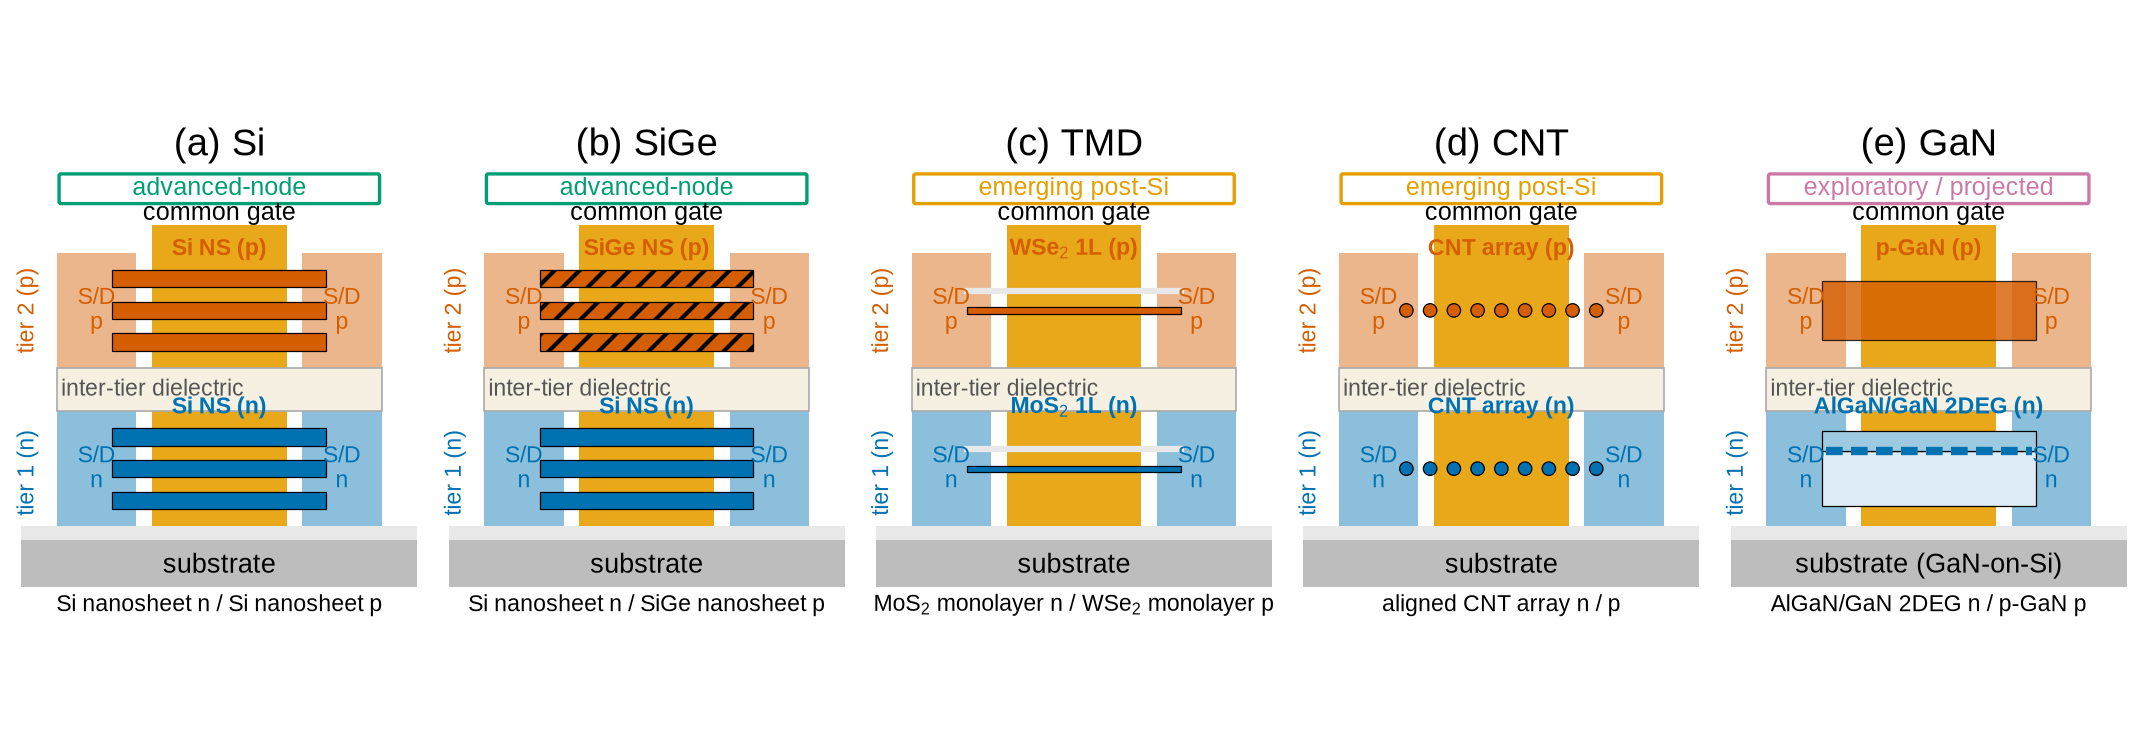
\includegraphics[width=\columnwidth]{fig01_cfet_stacks.png}
\caption{Cross-section cartoons of the five CFET platforms: bottom n-tier, inter-tier dielectric, top p-tier, common gate wrapping both tiers, and n/p source/drain contacts. Maturity tags follow Table~\ref{tab:platforms}.}
\label{fig:stacks}
\end{figure}

\section{Unified Compact Model}
\subsection{Core equations}
All nine devices share the four-terminal interface (d, g, s, b; b is a reference terminal tied to the source in every circuit) and internal nodes $d_i$, $s_i$ (series resistance) and $t_j$ (temperature rise). With $V_T = k_BT_{dev}/q$, the model uses an EKV-type smooth overdrive \cite{Enz1995}
\begin{equation}
V_{ov} = 2nV_T \ln\!\left[1+\exp\!\left(\frac{V_{GS}-V_{TH,eff}}{2nV_T}\right)\right],
\label{eq:vov}
\end{equation}
so that $V_{ov}^2 \propto \exp[(V_{GS}-V_{TH})/nV_T]$ in weak inversion (subthreshold slope $nV_T\ln 10$) and $V_{ov}\to V_{GS}-V_{TH}$ in strong inversion. Drain-induced barrier lowering enters as $V_{TH,eff} = V_{TH,T} - \eta\sqrt{V_{DS}^2+\delta^2}$ and the temperature dependence as $V_{TH,T} = V_{TH0}+k_{VTH}(T_{dev}-T_{nom})$, $\mu_T=\mu_0(T_{dev}/T_{nom})^{-m_\mu}$. The drift--diffusion branch with velocity saturation is
\begin{equation}
I_D = I_{sat}\tanh\!\left(\frac{2V_{DS}}{V_{dsat}}\right)\left(1+\lambda|V_{DS}|\right),\quad
I_{sat} = \frac{\beta V_{ov}^2}{2\left(1+\dfrac{V_{ov}}{V_{sat,v}}\right)},
\label{eq:id}
\end{equation}
with $\beta=\mu_T C_{ox,eff}W/L$, $V_{sat,v}=v_{sat}L/\mu_T$ and $V_{dsat}=V_{ov}/(1+V_{ov}/V_{sat,v})$. The factor 2 in the $\tanh$ argument makes the low-$V_{DS}$ conductance exactly $\beta V_{ov}$ while the saturation current retains the square law for long channels and the velocity-saturated limit $C_{ox}Wv_{sat}V_{ov}/2$ for short channels \cite{Lundstrom2002}; the function is odd in $V_{DS}$ and infinitely differentiable, which is what the Newton iterations of a circuit simulator need. Series resistances $R_S=R_{SW}/W$ and $R_D=R_{DW}/W$ act between the external and internal nodes.

\subsection{Terminal charges}
A DC-only model cannot produce RO frequencies. Terminal charges are defined per branch,
\begin{align}
Q_{gs} &= \tfrac12 WLC_{ox,eff}\,V_{ov}(V_{GS}) + C_{gso}WV_{GS},\\
Q_{gd} &= \tfrac12 WLC_{ox,eff}\,V_{ov}(V_{GD}) + C_{gdo}WV_{GD},
\end{align}
with $V_{ov}$ evaluated without DIBL so that each charge depends only on its own branch voltage, and injected as $I=\mathrm{d}Q/\mathrm{d}t$. With $Q_g=Q_{gs}+Q_{gd}$, $Q_s=-Q_{gs}$ and $Q_d=-Q_{gd}$, charge conservation $Q_g+Q_d+Q_s=0$ holds by construction; the symmetric source/drain-end partition reduces to 50/50 in the linear region and decouples the drain in saturation.

\subsection{Material blocks}
\emph{Si and SiGe nanosheets} use the core with $W_{eff}=N_{NS}\cdot 2(W_{NS}+T_{NS})$. \emph{MoS$_2$/WSe$_2$} add the quantum capacitance in series, $C_{ox,eff}=C_{ox}C_q/(C_{ox}+C_q)$, a trap-limited ideality $n=n_0(1+qD_{it}/C_{ox})$ and contact-dominated series resistance $R_{SW}=R_{DW}=R_C$ \cite{Pasadas2019,Li2023Nature}. \emph{CNT arrays} replace (\ref{eq:id}) by a Landauer quasi-ballistic branch \cite{Deng2007,Lundstrom2002}
\begin{equation}
I_D = N_{tube}\,G_0 T\, nV_T\!\left[F(\eta_s)-F\!\left(\eta_s-\tfrac{V_{DS}}{nV_T}\right)\right](1+\lambda|V_{DS}|) + G_{met}V_{DS},
\end{equation}
with $F(x)=\ln(1+e^x)$, $\eta_s=\alpha(V_{GS}-V_{TH,eff})/nV_T$, $G_0=4q^2/h$, $N_{tube}=D_{CNT}W(1-F_{met})$ and the metallic-tube shunt $G_{met}=F_{met}D_{CNT}WG_0T$. \emph{GaN} adds an electro-thermal node: $I(t_j)=-I_DV_{DS}+V(t_j)/R_{th}+C_{th}\,\mathrm{d}V(t_j)/\mathrm{d}t$ and $T_{dev}=T_{amb}+V(t_j)$, i.e.\ the quasi-static self-heating $T_{dev}=T_{amb}+R_{th}P_{diss}$ with a thermal time constant $R_{th}C_{th}$.

\subsection{Implementation and equivalence}
The nine Verilog-A modules (\texttt{gaa\_n}, \texttt{gaa\_p}, \texttt{sige\_p}, \texttt{mos2\_n}, \texttt{wse2\_p}, \texttt{cnt\_n}, \texttt{cnt\_p}, \texttt{gan\_n}, \texttt{gan\_p}) are generated from one parameter table, as is an ngspice behavioural library in which the same equations are evaluated by B-sources, \texttt{.func} macros and charge-based ($Q=$) capacitors; intermediate quantities ($V_{ov}$, $V_{dsat}$, $\eta_s$) are solved on auxiliary nodes, which speeds the transient analysis by $7\times$ without changing the result. A NumPy reference implementation is used for calibration. DC sweeps of all nine devices agree between ngspice and the reference implementation to within 0.1\% (the residual is the tolerance of the bisection used for the series-resistance loop). Spectre was not available in the computing environment used for this paper; the Cadence SKILL/OCEAN/ADE scripts that build the library, symbols, schematics and analyses are provided and documented step by step, and all manuscript results were generated with the ngspice mirror.

\section{Calibration}
\begin{figure*}[!t]
\centering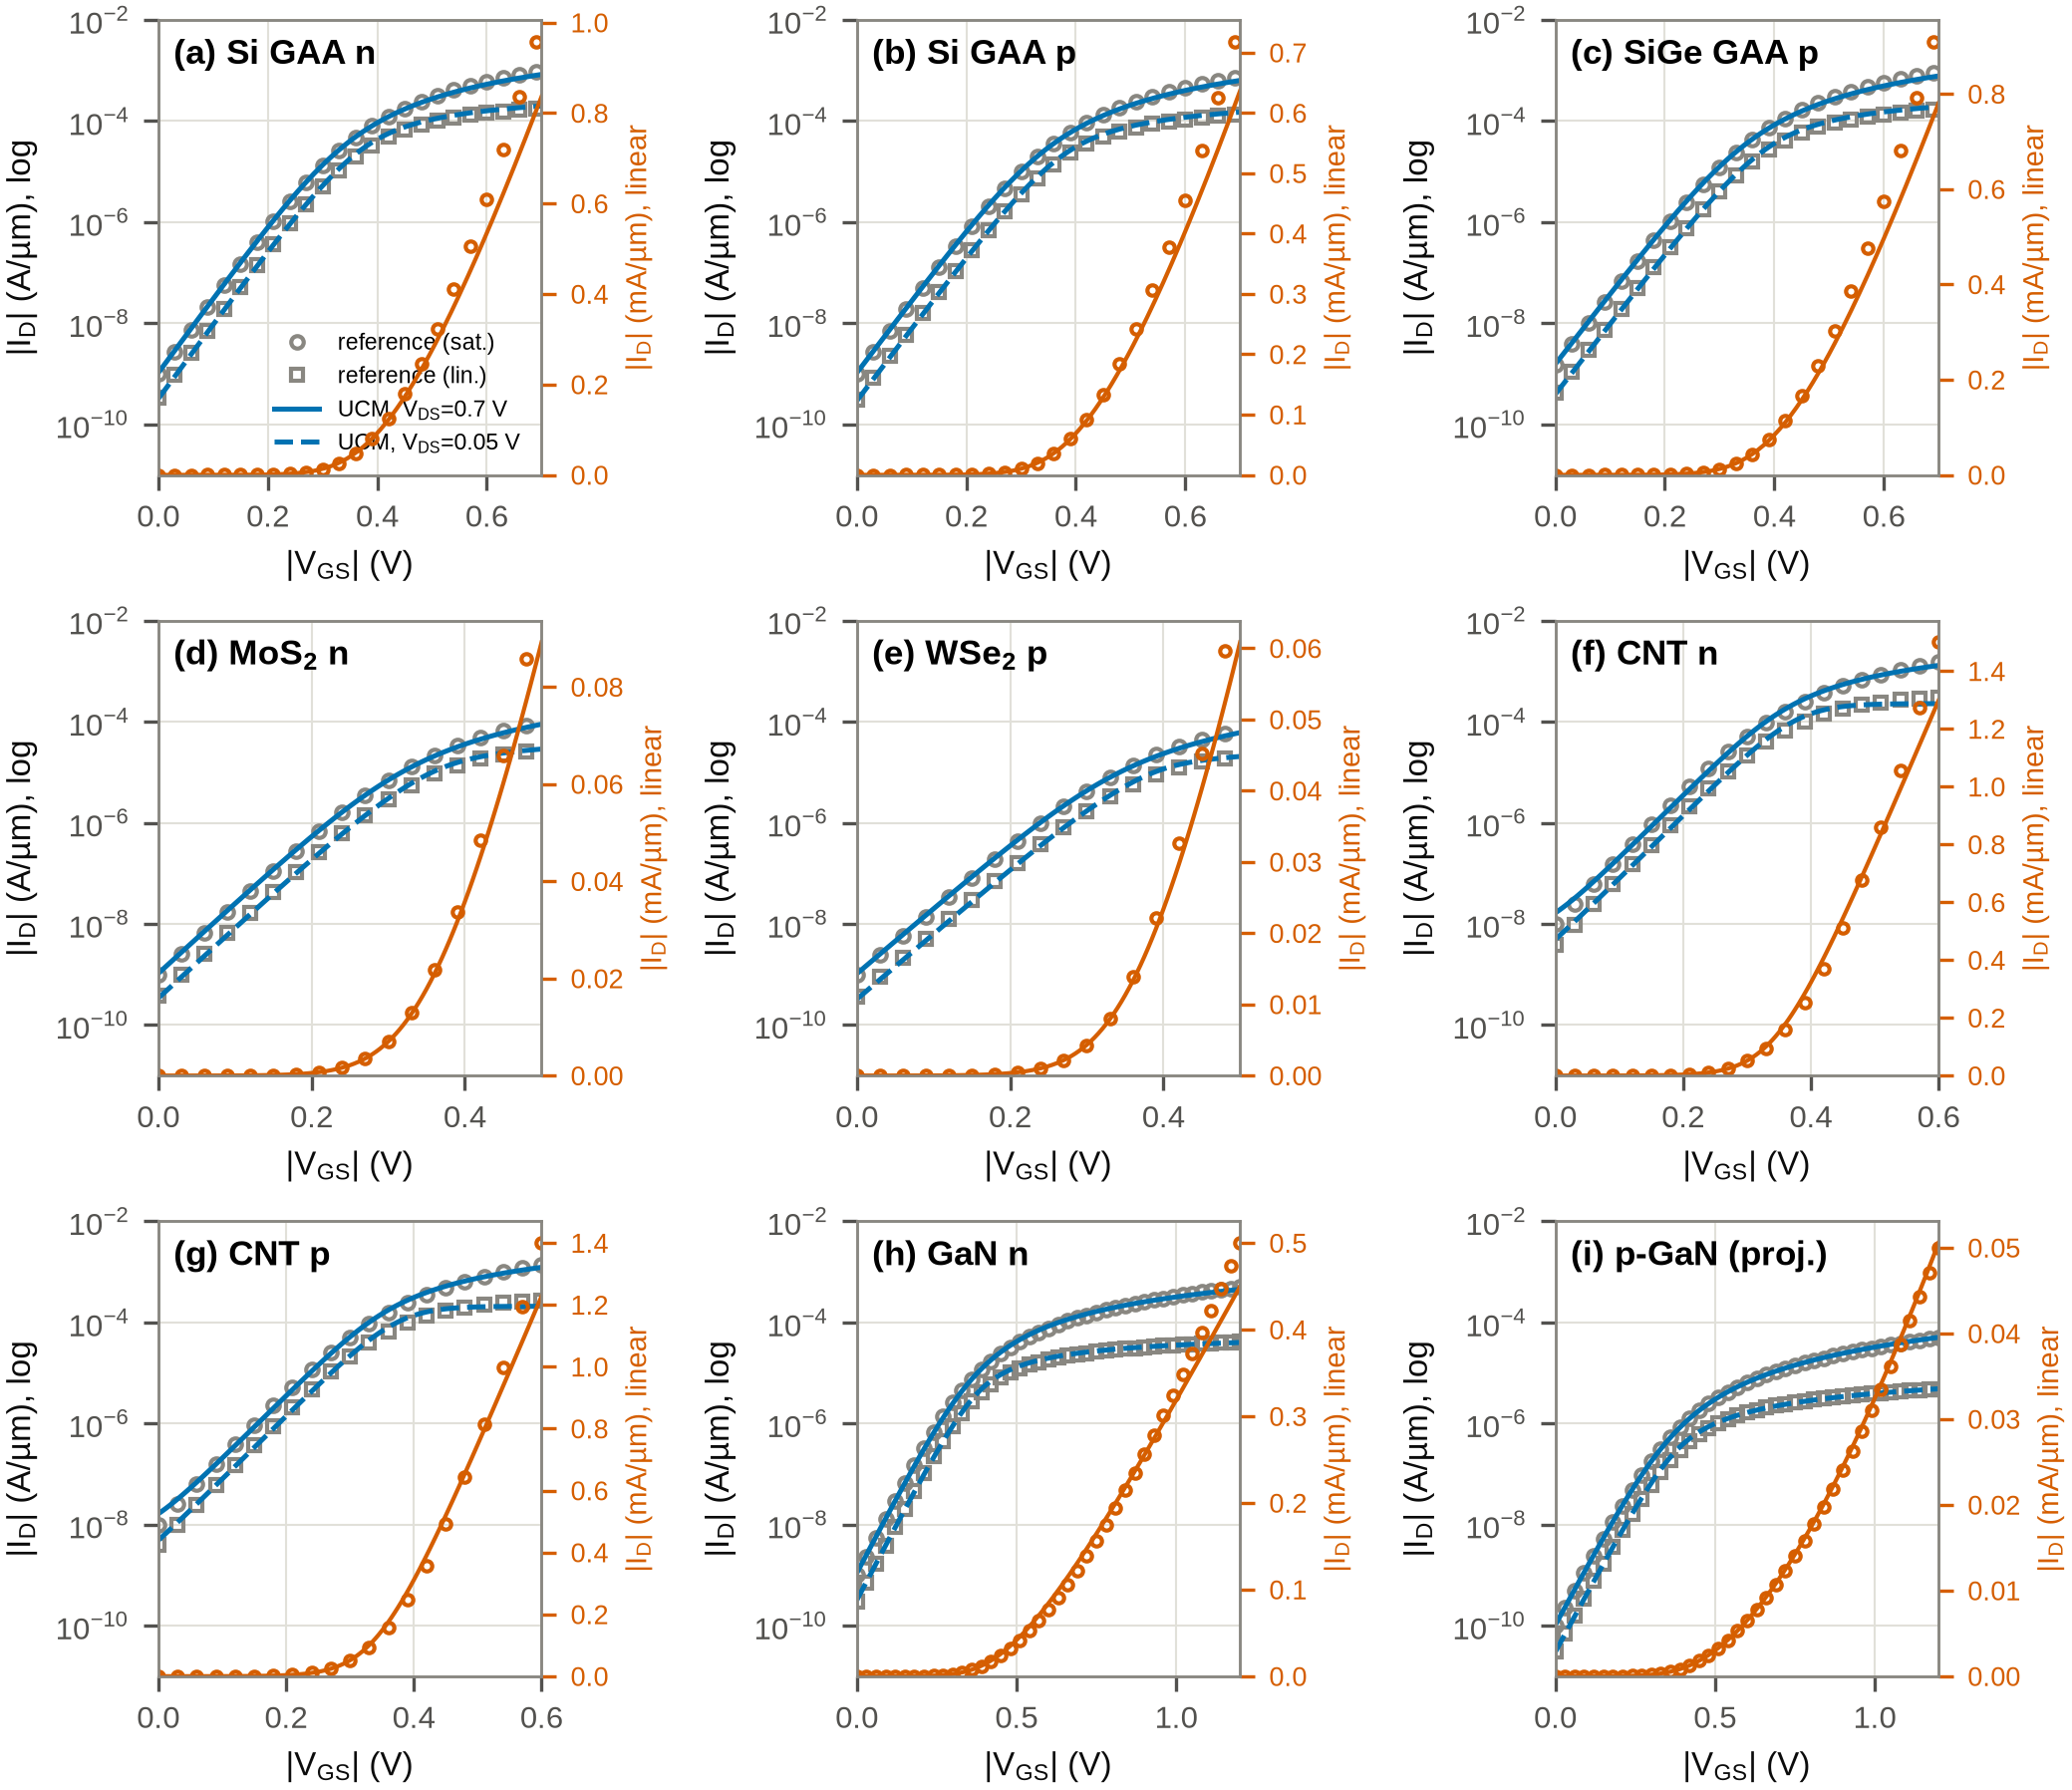
\includegraphics[width=\textwidth]{fig02_calibration_idvg.png}
\caption{$I_D$--$V_G$ calibration of the nine device models (lines) against the literature-anchored reference curves (symbols) at $|V_{DS}|=0.05$~V and $|V_{DS}|=V_{DD}$, on logarithmic (left axes) and linear (right axes) scales.}
\label{fig:idvg}
\end{figure*}
\begin{figure*}[!t]
\centering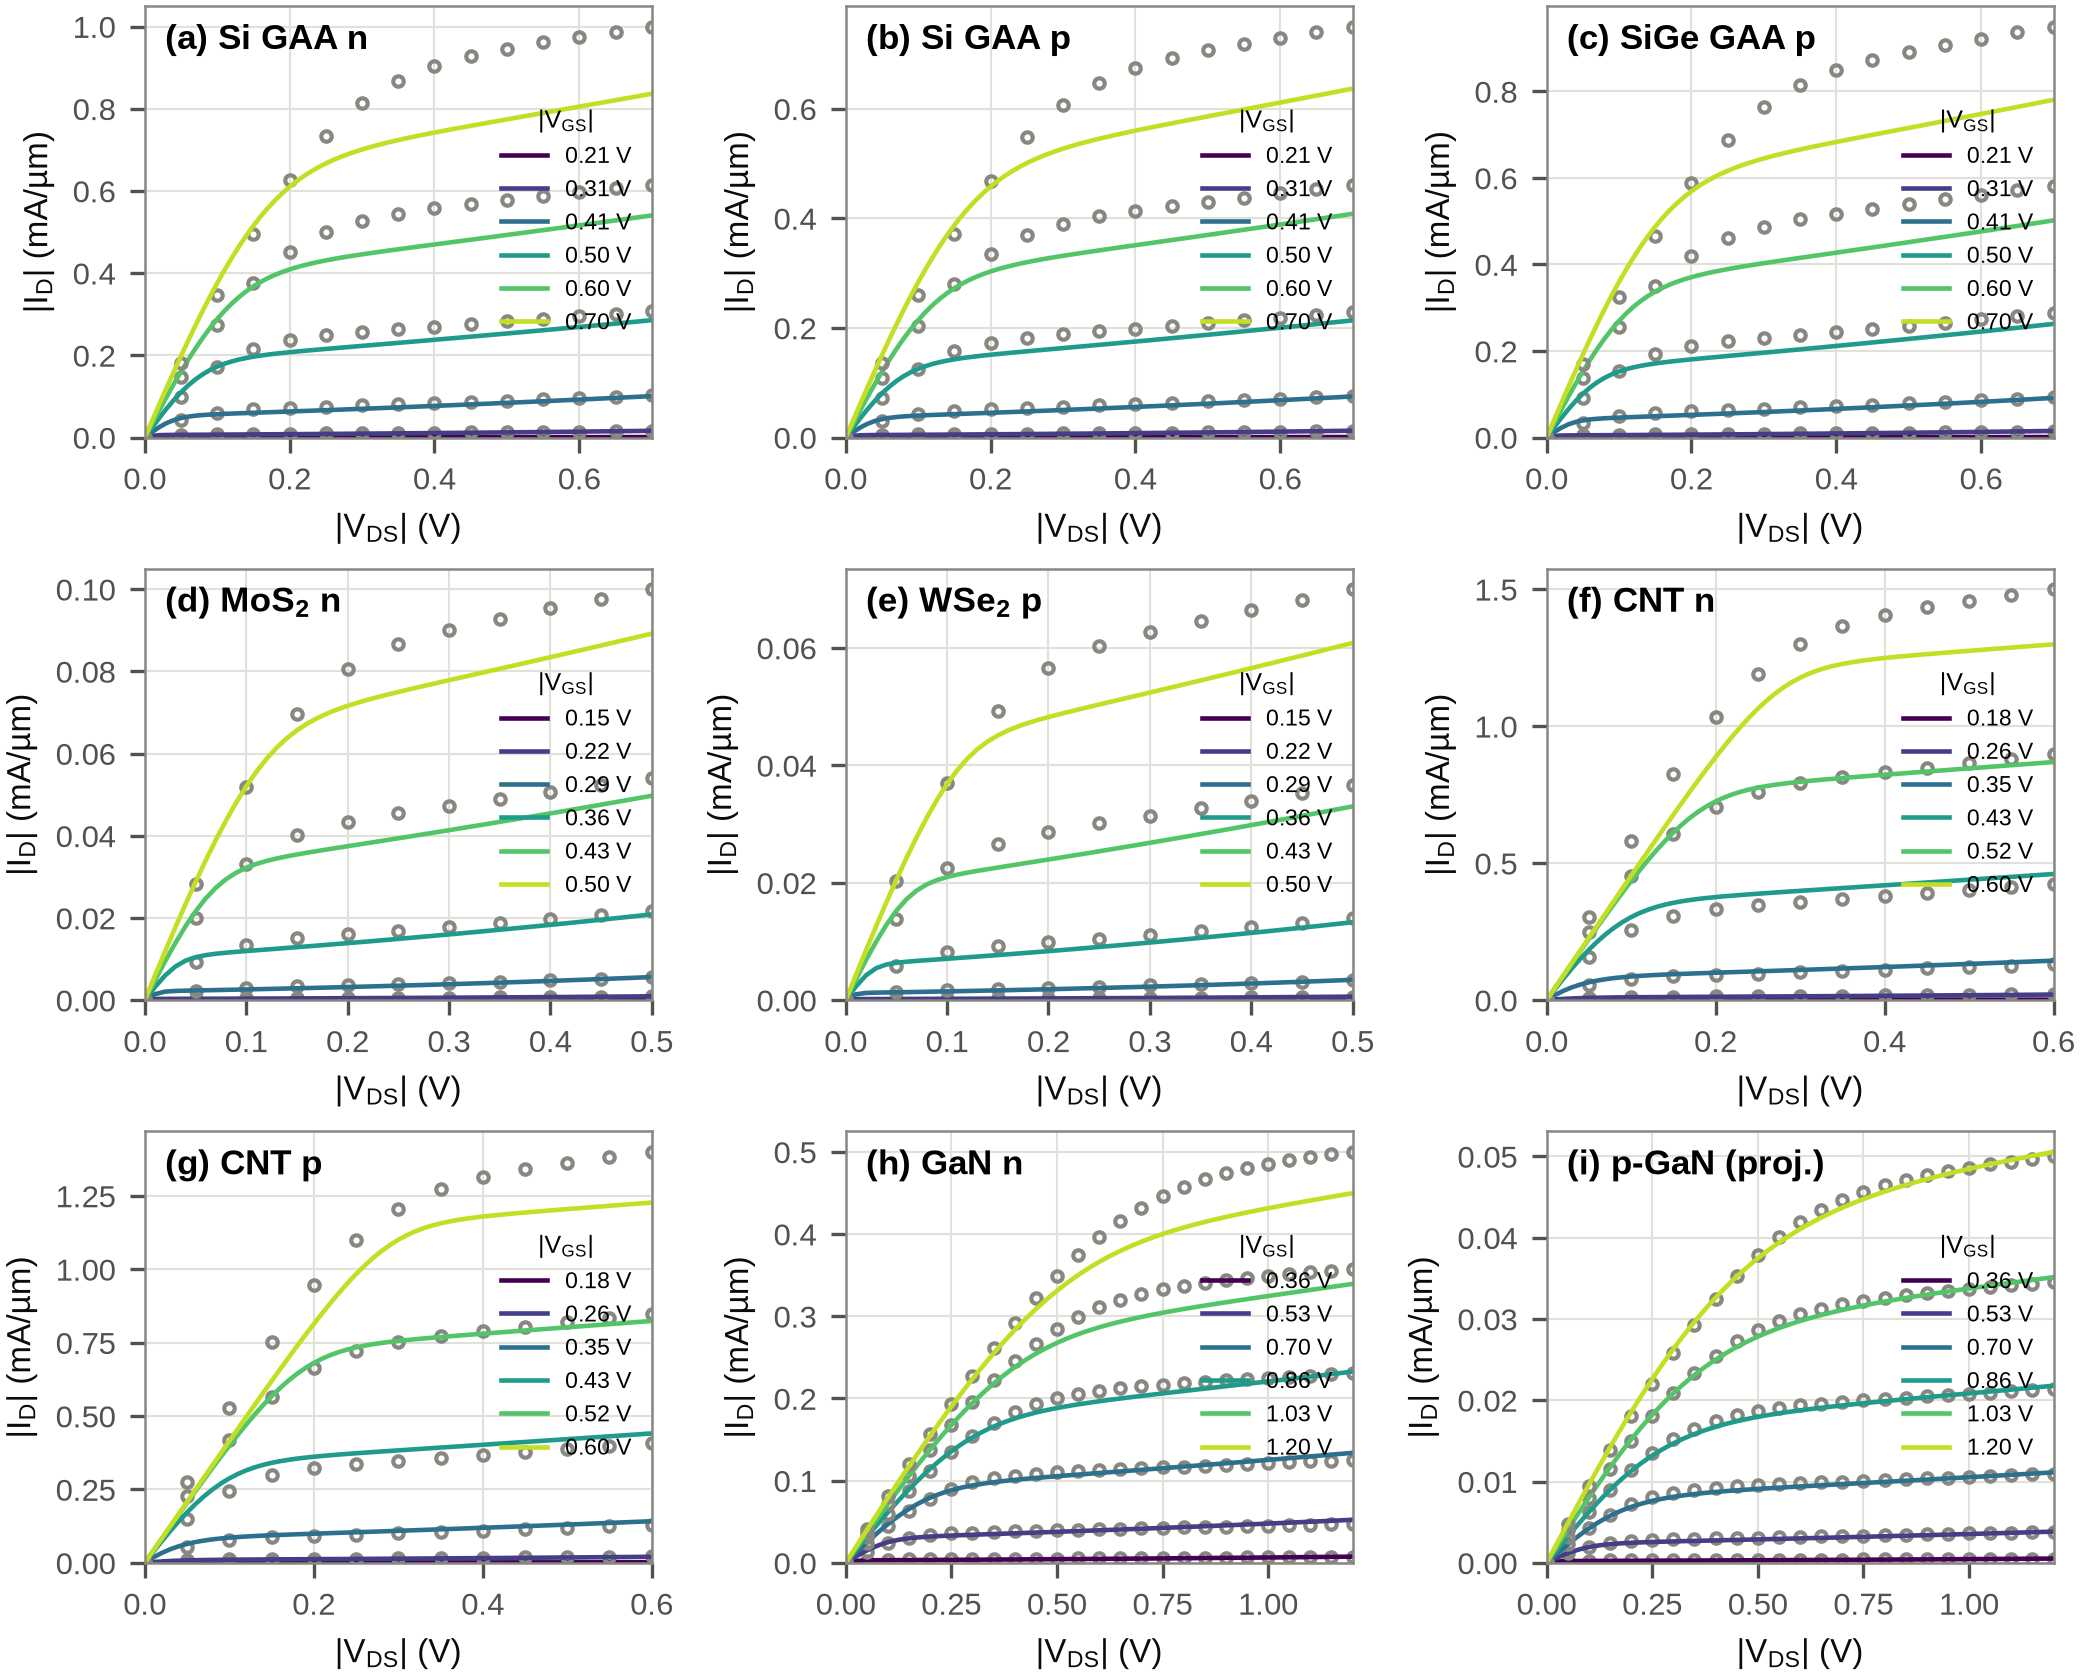
\includegraphics[width=\textwidth]{fig03_calibration_idvd.png}
\caption{$I_D$--$V_D$ families (six gate biases from $0.3V_{DD}$ to $V_{DD}$) of the calibrated models (lines) and reference (symbols).}
\label{fig:idvd}
\end{figure*}
No measured or TCAD data were available, so the calibration targets are literature-anchored synthetic reference curves: for each device the on-current, off-current, subthreshold slope and DIBL at the platform $V_{DD}$ (Table~\ref{tab:devparams}, sources in the companion \texttt{doc/calibration\_targets.md}) are imposed on an \emph{independent} EKV-type formulation with a fourth-order power-law drain-voltage smoothing and explicit series resistance; the UCM is then fitted to those curves. This makes the fit a real test of the model's functional form (the two formulations differ in their saturation behaviour and charge interpolation), while keeping the targets traceable to published ranges \cite{IRDS2023,Loubet2017,Mertens2016,Mochizuki2020,Li2023Nature,Shen2021,Chou2022,Liu2020Science,Amano2018,Bader2020}. The flow accepts measured or TCAD CSV files with the same column layout as drop-in replacements.

Seven parameters are fitted per device by bounded non-linear least squares on $\log_{10}I_D$ of the linear and saturation $I_D$--$V_G$ curves and on the relative error of the $I_D$--$V_D$ family: $V_{TH0}$, $\mu_0$ (transmission $T$ and gate efficiency $\alpha$ for CNT), $v_{sat}$, $R_{SW}=R_{DW}$ (Si, SiGe, GaN only), $\lambda$, $\eta$ and $n_0$. The 2D and CNT contact resistances are held at their physical nominal values because they are measured quantities in practice and are the subject of the sensitivity study. Figs.~\ref{fig:idvg}--\ref{fig:mape} and Table~\ref{tab:calibration} summarise the result: the mean absolute percentage error (MAPE) is \mapeIdVgMin--\mapeIdVgMax\% on $I_D$--$V_G$ and \mapeIdVdMin--\mapeIdVdMax\% on the $I_D$--$V_D$ families, with the on/off currents within 20\% and the subthreshold slopes within 3~mV/dec of their targets. The largest residuals are in the SiGe/Si output conductance (the $\tanh$ interpolation saturates harder than the reference, which the fit compensates with $\lambda$ at its 0.3~V$^{-1}$ bound) and in the CNT subthreshold region, where the single-ideality Landauer branch cannot reproduce the reference's 75~mV/dec slope together with its DIBL.
\begin{table*}[!t]
\caption{Calibrated \ucm\ parameters (SI values converted to the units shown).}
\label{tab:devparams}
\centering\scriptsize
\begin{tabular}{lrrrrrrrrr}
\hline
Parameter & Si GAA n & Si GAA p & SiGe GAA p & MoS$_2$ n & WSe$_2$ p & CNT n & CNT p & GaN n & p-GaN (proj.) \\
\hline
$L_g$ (nm) & 16 & 16 & 16 & 20 & 20 & 20 & 20 & 100 & 100 \\
$V_{TH0}$ (mV) & 346 & 350 & 362 & 343 & 380 & 377 & 375 & 357 & 355 \\
$n_0$ & 1.14 & 1.17 & 1.20 & 1.18 & 1.24 & 1.16 & 1.15 & 1.39 & 1.43 \\
$\eta$ (mV/V) & 46 & 51 & 57 & 70 & 77 & 46 & 46 & 33 & 37 \\
$\mu_0$ (cm$^2$/Vs) & 75 & 55 & 76 & 56 & 63 & -- & -- & 300 & 19 \\
$v_{sat}$ ($10^7$ cm/s) & 2.50 & 2.00 & 2.25 & 1.50 & 1.20 & -- & -- & 3.75 & 1.25 \\
$\lambda$ (V$^{-1}$) & 0.30 & 0.30 & 0.30 & 0.30 & 0.30 & 0.00 & 0.00 & 0.19 & 0.08 \\
$R_{S}W$ ($\Omega\cdot\mu$m) & 53 & 65 & 55 & 500 & 800 & 50 & 60 & 374 & 1213 \\
$C_{ox}$ (fF/$\mu$m$^2$) & 43.0 & 43.0 & 43.0 & 34.5 & 34.5 & 20.0 & 20.0 & 8.0 & 8.0 \\
$C_{gso}$ (fF/$\mu$m) & 0.30 & 0.30 & 0.32 & 0.20 & 0.20 & 0.15 & 0.15 & 0.50 & 0.50 \\
$W_{eff}$ (nm) & 150 & 150 & 150 & 100 & 100 & 100 & 100 & 1000 & 3000 \\
material block & -- & -- & -- & $C_q$=1.2, $D_{it}$=5e+11 & $C_q$=1.1, $D_{it}$=1e+12 & $T$=0.22, $\alpha$=0.86 & $T$=0.21, $\alpha$=0.86 & $R_{th}$=1.5e5 & $R_{th}$=1.0e5 \\
\hline
\end{tabular}

\end{table*}
\begin{table*}[!t]
\caption{Calibration error and figures of merit (model vs. reference).}
\label{tab:calibration}
\centering\scriptsize
\begin{tabular}{lrrrrrrrrr}
\hline
Device & MAPE$_{lin}$ & MAPE$_{sat}$ & MAPE$_{I_D\text{-}V_D}$ & $I_{ON}$ & $I_{ON}^{ref}$ & $I_{OFF}$ & SS & SS$^{ref}$ & DIBL \\
 & (\%) & (\%) & (\%) & (mA/$\mu$m) & (mA/$\mu$m) & (nA/$\mu$m) & (mV/dec) & (mV/dec) & (mV/V) \\
\hline
Si GAA n & 8.1 & 6.0 & 10.8 & 0.84 & 1.00 & 1.05 & 68 & 68 & 54 \\
Si GAA p & 7.9 & 5.8 & 10.7 & 0.64 & 0.75 & 1.05 & 70 & 70 & 60 \\
SiGe GAA p & 8.7 & 7.0 & 11.9 & 0.78 & 0.95 & 1.56 & 72 & 72 & 66 \\
MoS$_2$ n & 6.7 & 5.1 & 11.2 & 0.09 & 0.10 & 1.05 & 72 & 72 & 79 \\
WSe$_2$ p & 6.9 & 6.1 & 12.6 & 0.06 & 0.07 & 1.03 & 77 & 78 & 87 \\
CNT n & 12.1 & 10.2 & 9.9 & 1.30 & 1.50 & 16.52 & 86 & 75 & 62 \\
CNT p & 11.6 & 9.7 & 9.4 & 1.23 & 1.40 & 16.34 & 85 & 75 & 62 \\
GaN n & 5.1 & 5.2 & 5.7 & 0.45 & 0.50 & 1.10 & 83 & 81 & 39 \\
p-GaN (proj.) & 3.0 & 1.3 & 3.7 & 0.05 & 0.05 & 0.10 & 86 & 86 & 41 \\
\hline
\end{tabular}

\end{table*}
\begin{figure}[!t]
\centering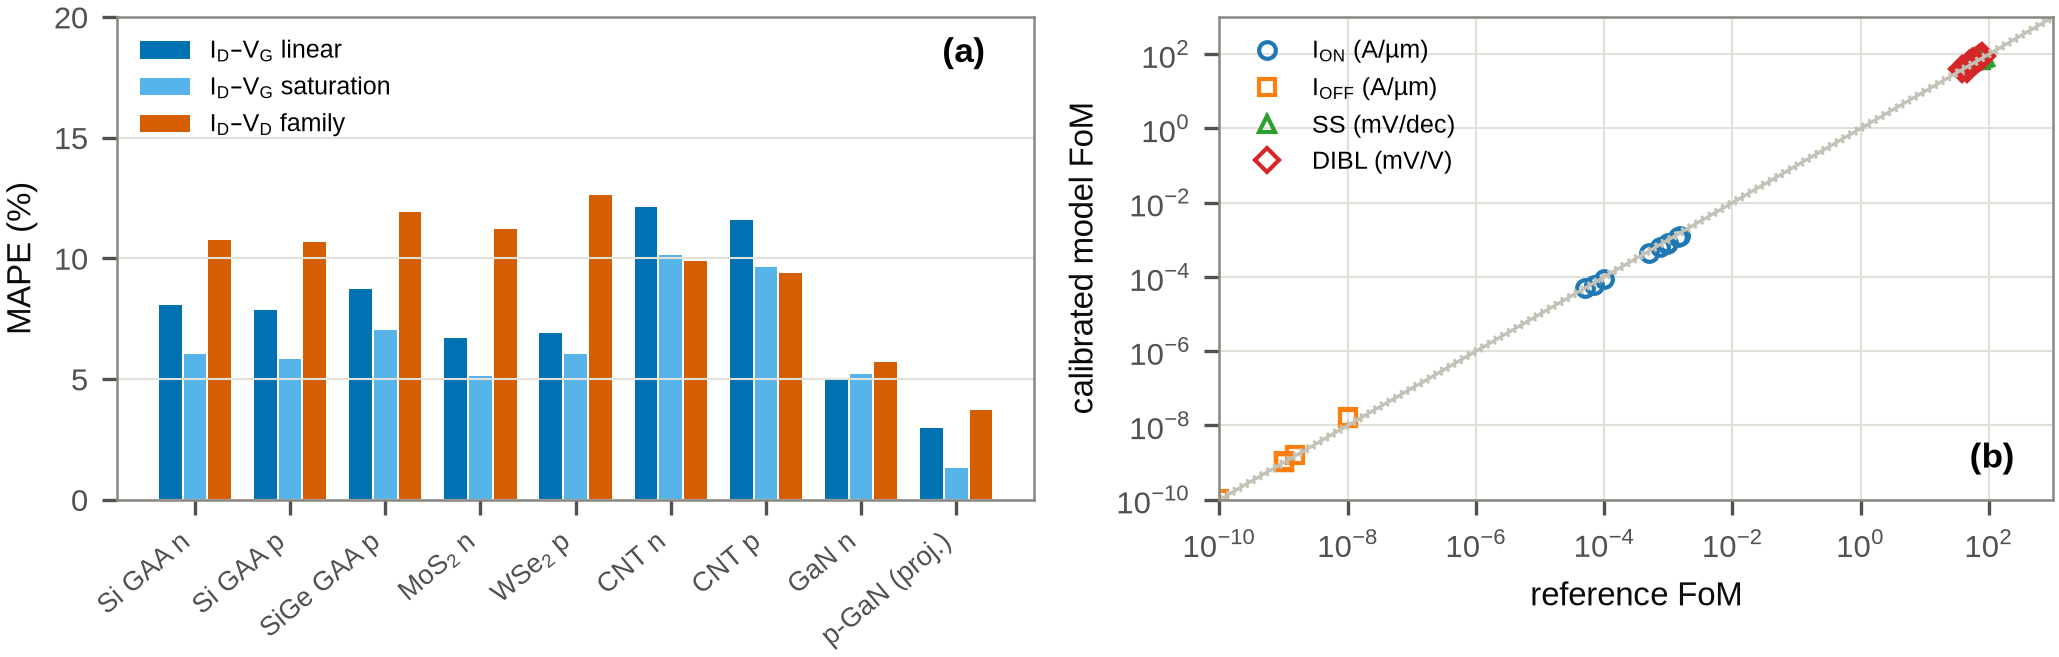
\includegraphics[width=\columnwidth]{fig04_calibration_mape.png}
\caption{(a) MAPE per device and data set; (b) parity of model vs. reference figures of merit.}
\label{fig:mape}
\end{figure}

\section{Circuit-Validation Flow}
\begin{figure}[!t]
\centering
\subfloat[]{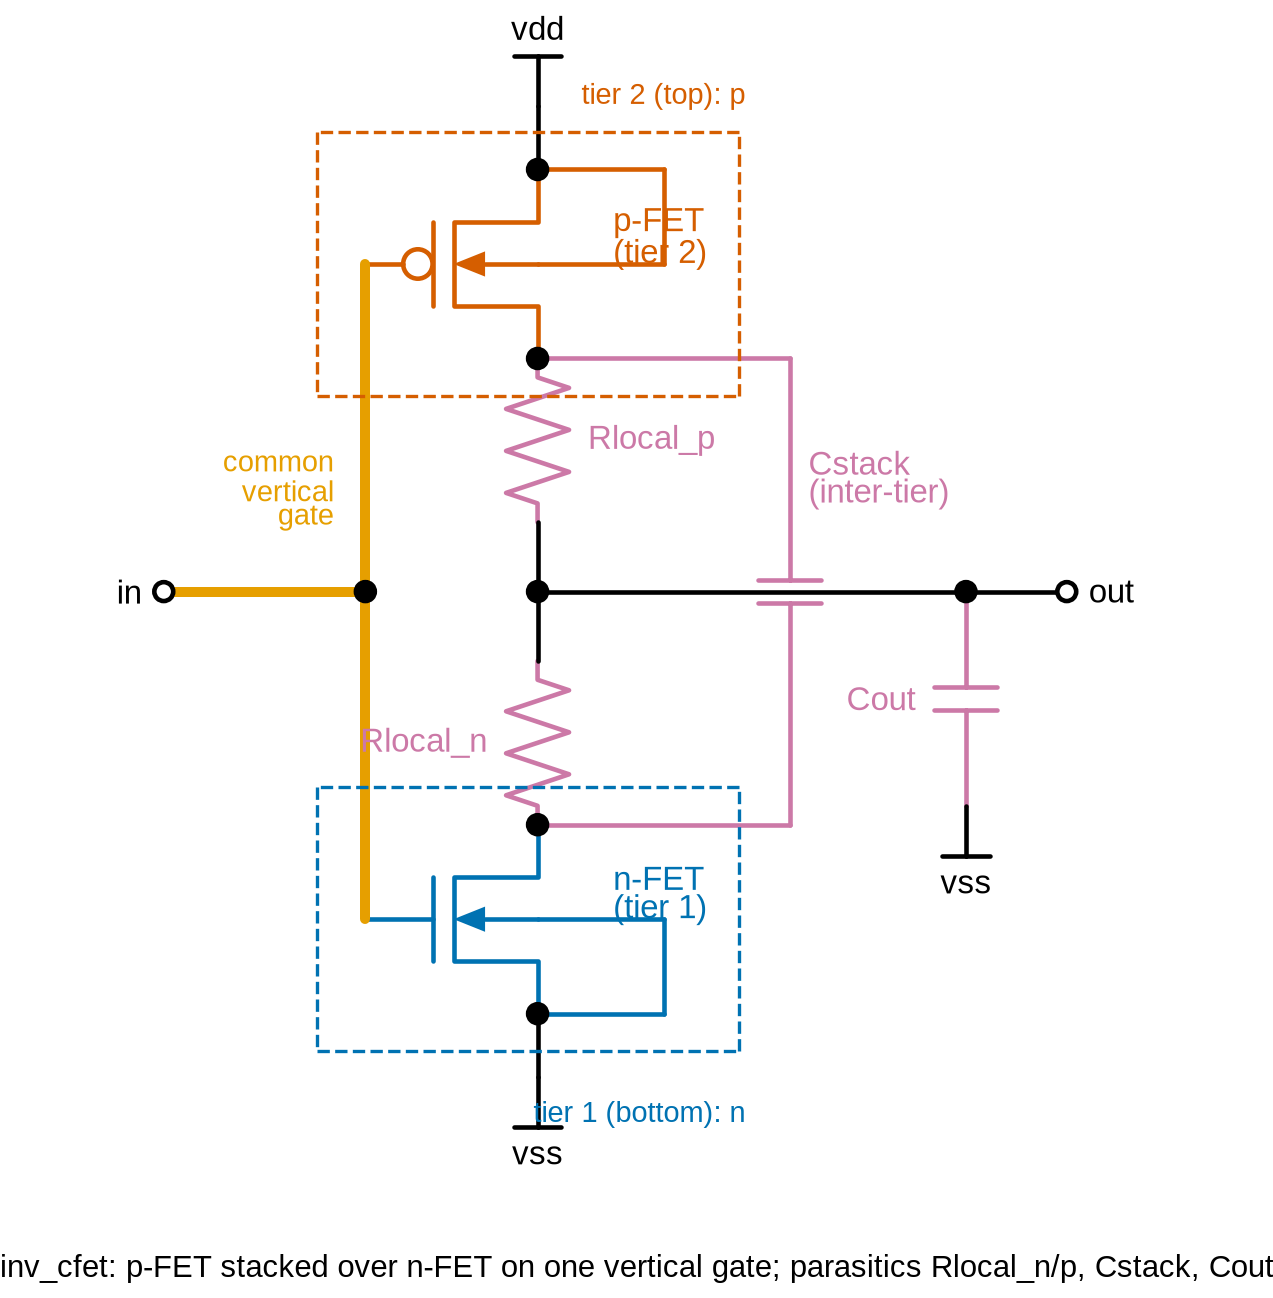
\includegraphics[width=0.48\columnwidth]{inv_cfet.png}}\hfil
\subfloat[]{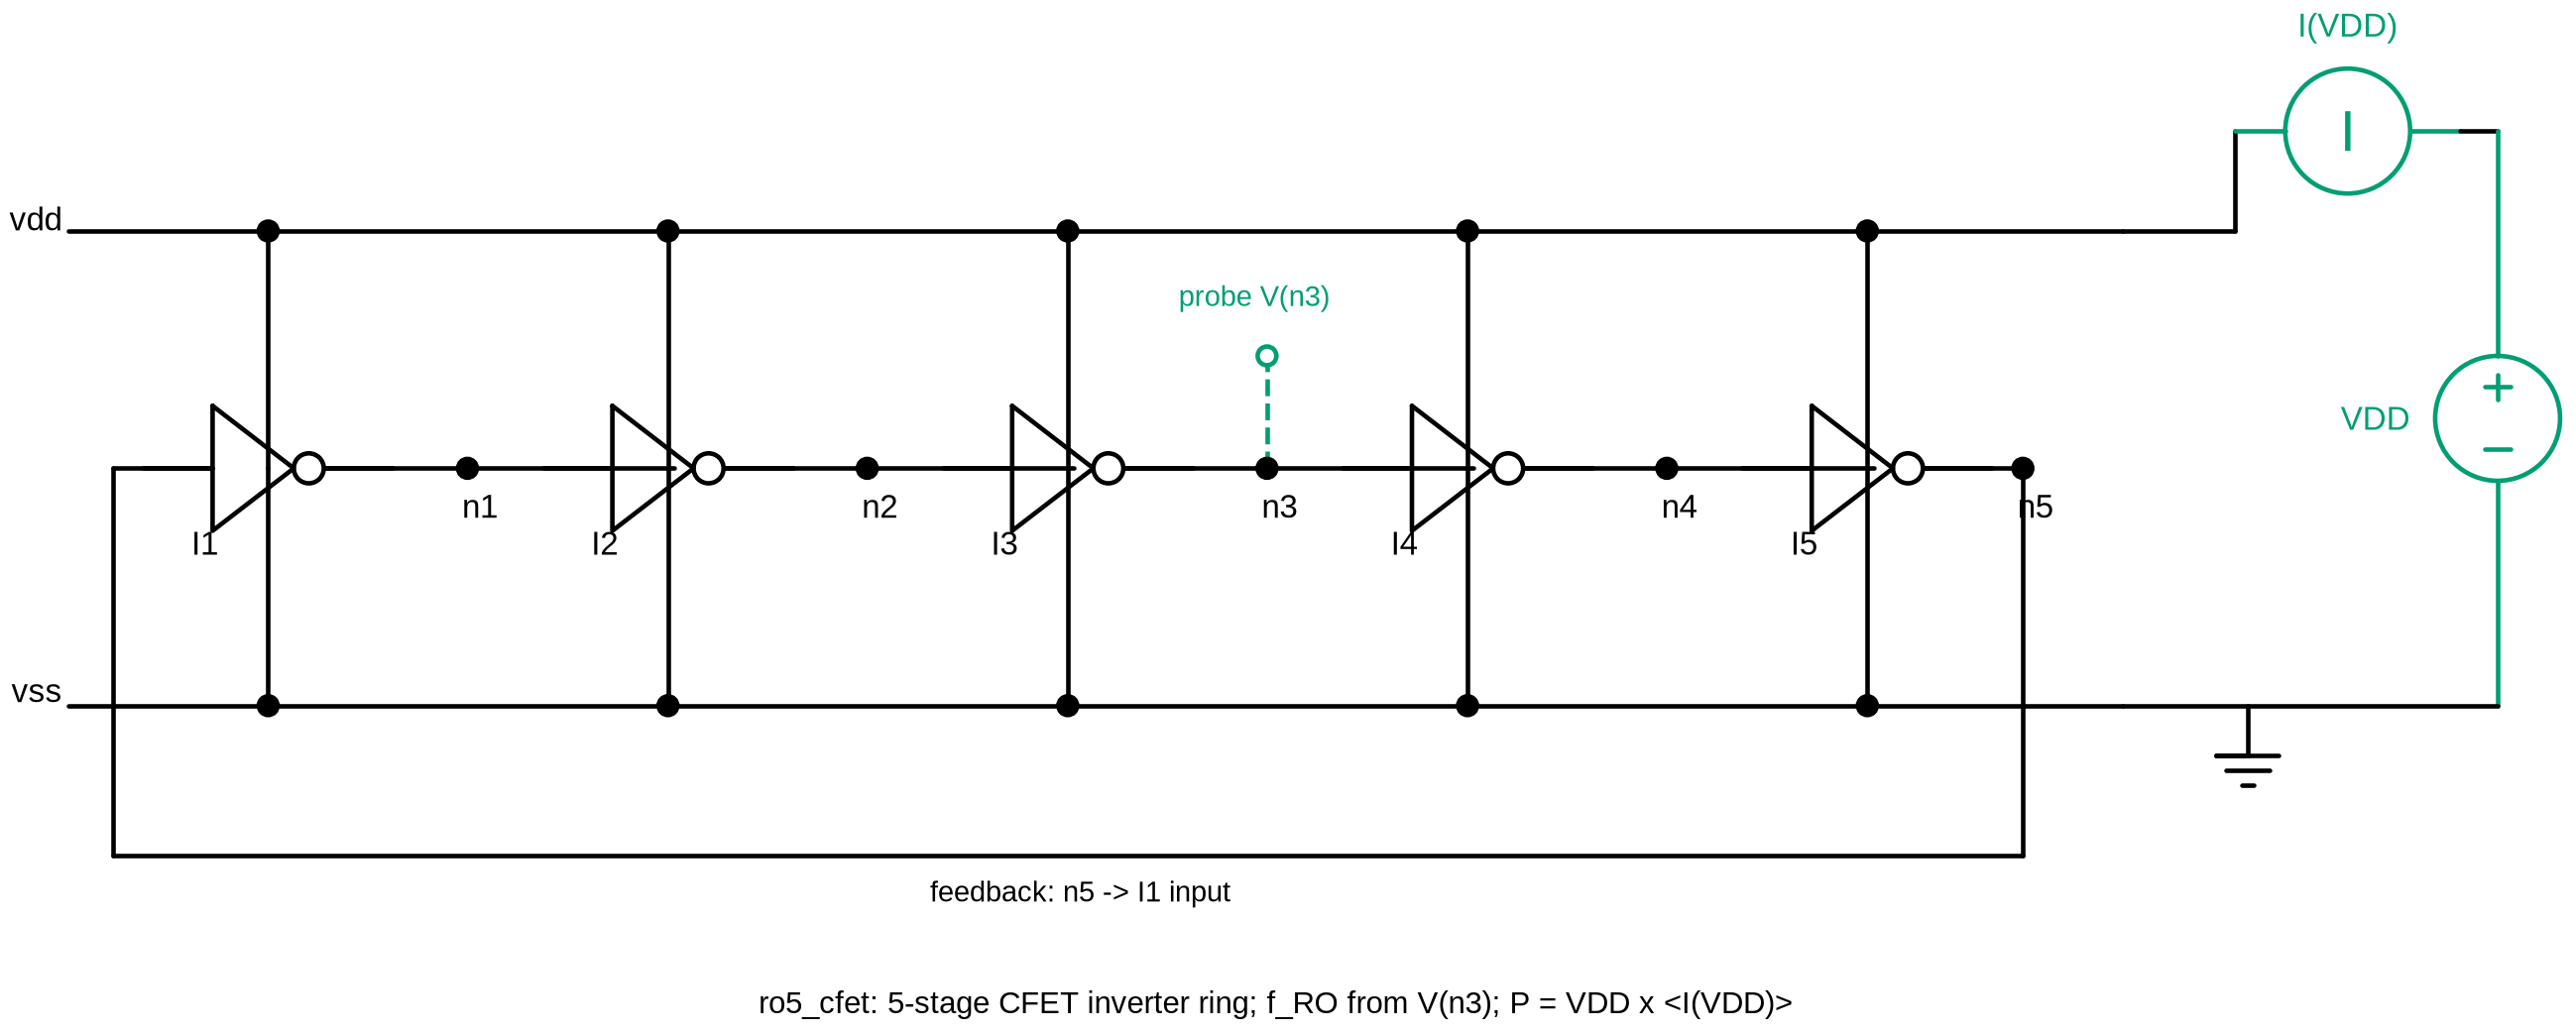
\includegraphics[width=0.48\columnwidth]{ro5_cfet.png}}
\caption{(a) CFET inverter cell with the explicit inter-tier coupling capacitance $C_{stack}$, output parasitic $C_{out}$ and local-interconnect resistances $R_{local,n/p}$; (b) 5-stage ring oscillator testbench with the $V(n_3)$ probe and the $I(V_{DD})$ meter.}
\label{fig:schem}
\end{figure}
\subsection{Testbenches}
The electrical inverter (Fig.~\ref{fig:schem}a) is a conventional CMOS inverter; its CFET interpretation is carried by the parasitic network: $C_{stack}$ between the n- and p-tier drain nodes, $C_{out}$ from the output to $V_{SS}$ and $R_{local,n/p}$ in the two drain legs. These are design variables (0.05/0.3~fF/10~$\Omega$ for Si and SiGe, 0.03/0.3~fF/50~$\Omega$ for TMD and CNT, 0.1/1~fF/20~$\Omega$ for GaN, each the mid-value of the ranges in Section~II of the flow definition). The same five inverter cells are used for the VTC (DC sweep of $V_{in}$ from 0 to $V_{DD}$: switching voltage $V_M$, maximum gain $A_V$, noise margins from the unity-gain points, static supply current), the transient delay (pulse 0$\to V_{DD}$, 100~ps delay, 5~ps edges, 500~ps width, 1~ns period, $C_{load}$ = 0.3~fF or 1~fF for GaN; $t_{pHL}$, $t_{pLH}$ at the 50\% crossings; switching energy $\int V_{DD}I_{DD}\mathrm{d}t$ over one period) and the $N$-stage ROs (Fig.~\ref{fig:schem}b).

\subsection{Ring-oscillator measurement}
Oscillation is started identically for every platform by an initial condition $V(n_1)=0$ together with a stated 1\% width increase of the stage-1 p-FET. A two-pass transient is used: a coarse pass, sized from the inverter delay ($T\approx 2Nt_{pd}$), pins down the period $T$; the fine pass then runs with a maximum step of $T/300$ and the frequency is measured from the rising $V_{DD}/2$ crossings of $V(n_3)$ between cycles 10 and 30 (the cycle 10--11 value is also recorded and differs by $<0.01$\%). For GaN the measurement window starts only after five thermal time constants, so that the steady-state self-heating is included. From $f_{RO}$ the stage delay $t_{pd}=1/(2Nf_{RO})$, the average power $P_{avg}=\frac{1}{t_2-t_1}\int_{t_1}^{t_2}V_{DD}I_{DD}\mathrm{d}t$ over the same window, $E_{cycle}=P_{avg}/f_{RO}$ and $\mathrm{PDP}=P_{avg}t_{pd}$ follow. Identical window definitions are used for all materials. The ADE Explorer/Assembler equivalents (OCEAN scripts with \texttt{cross}, \texttt{delay}, \texttt{integ} and \texttt{average} calculator functions, parametric sweeps, corners and Monte Carlo sampling) are provided in the companion \texttt{cadence/} directory.

\section{Results}
\subsection{Nominal inverters and ring oscillators}
\begin{figure}[!t]
\centering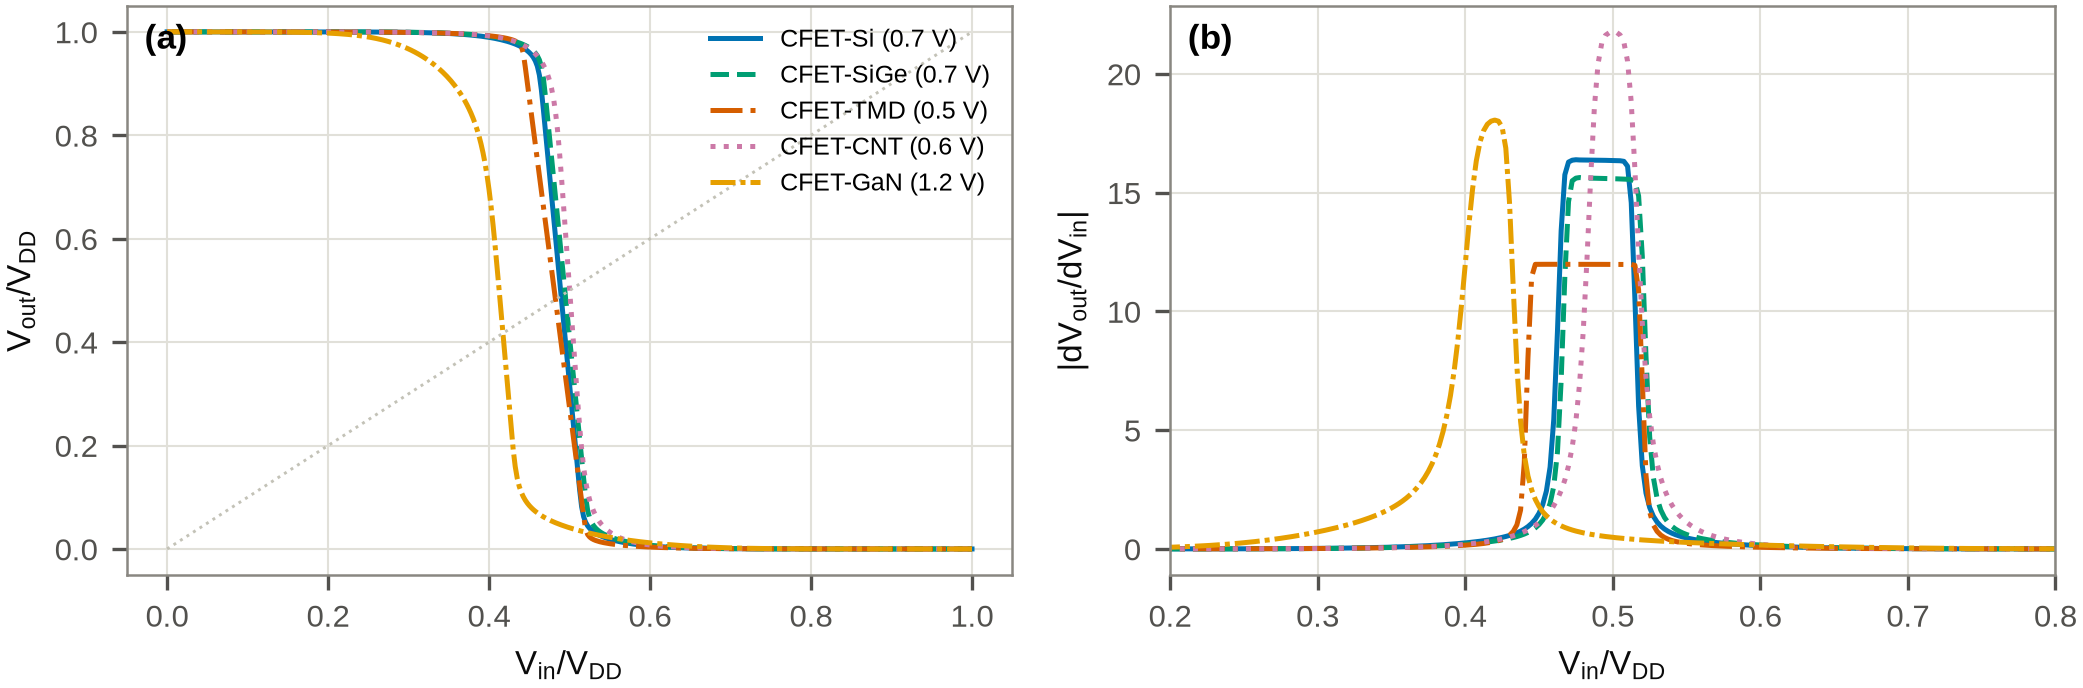
\includegraphics[width=\columnwidth]{fig05_inverter_vtc.png}
\caption{(a) Normalised voltage-transfer characteristics of the five CFET inverters at their nominal $V_{DD}$; (b) small-signal gain.}
\label{fig:vtc}
\end{figure}
\begin{figure}[!t]
\centering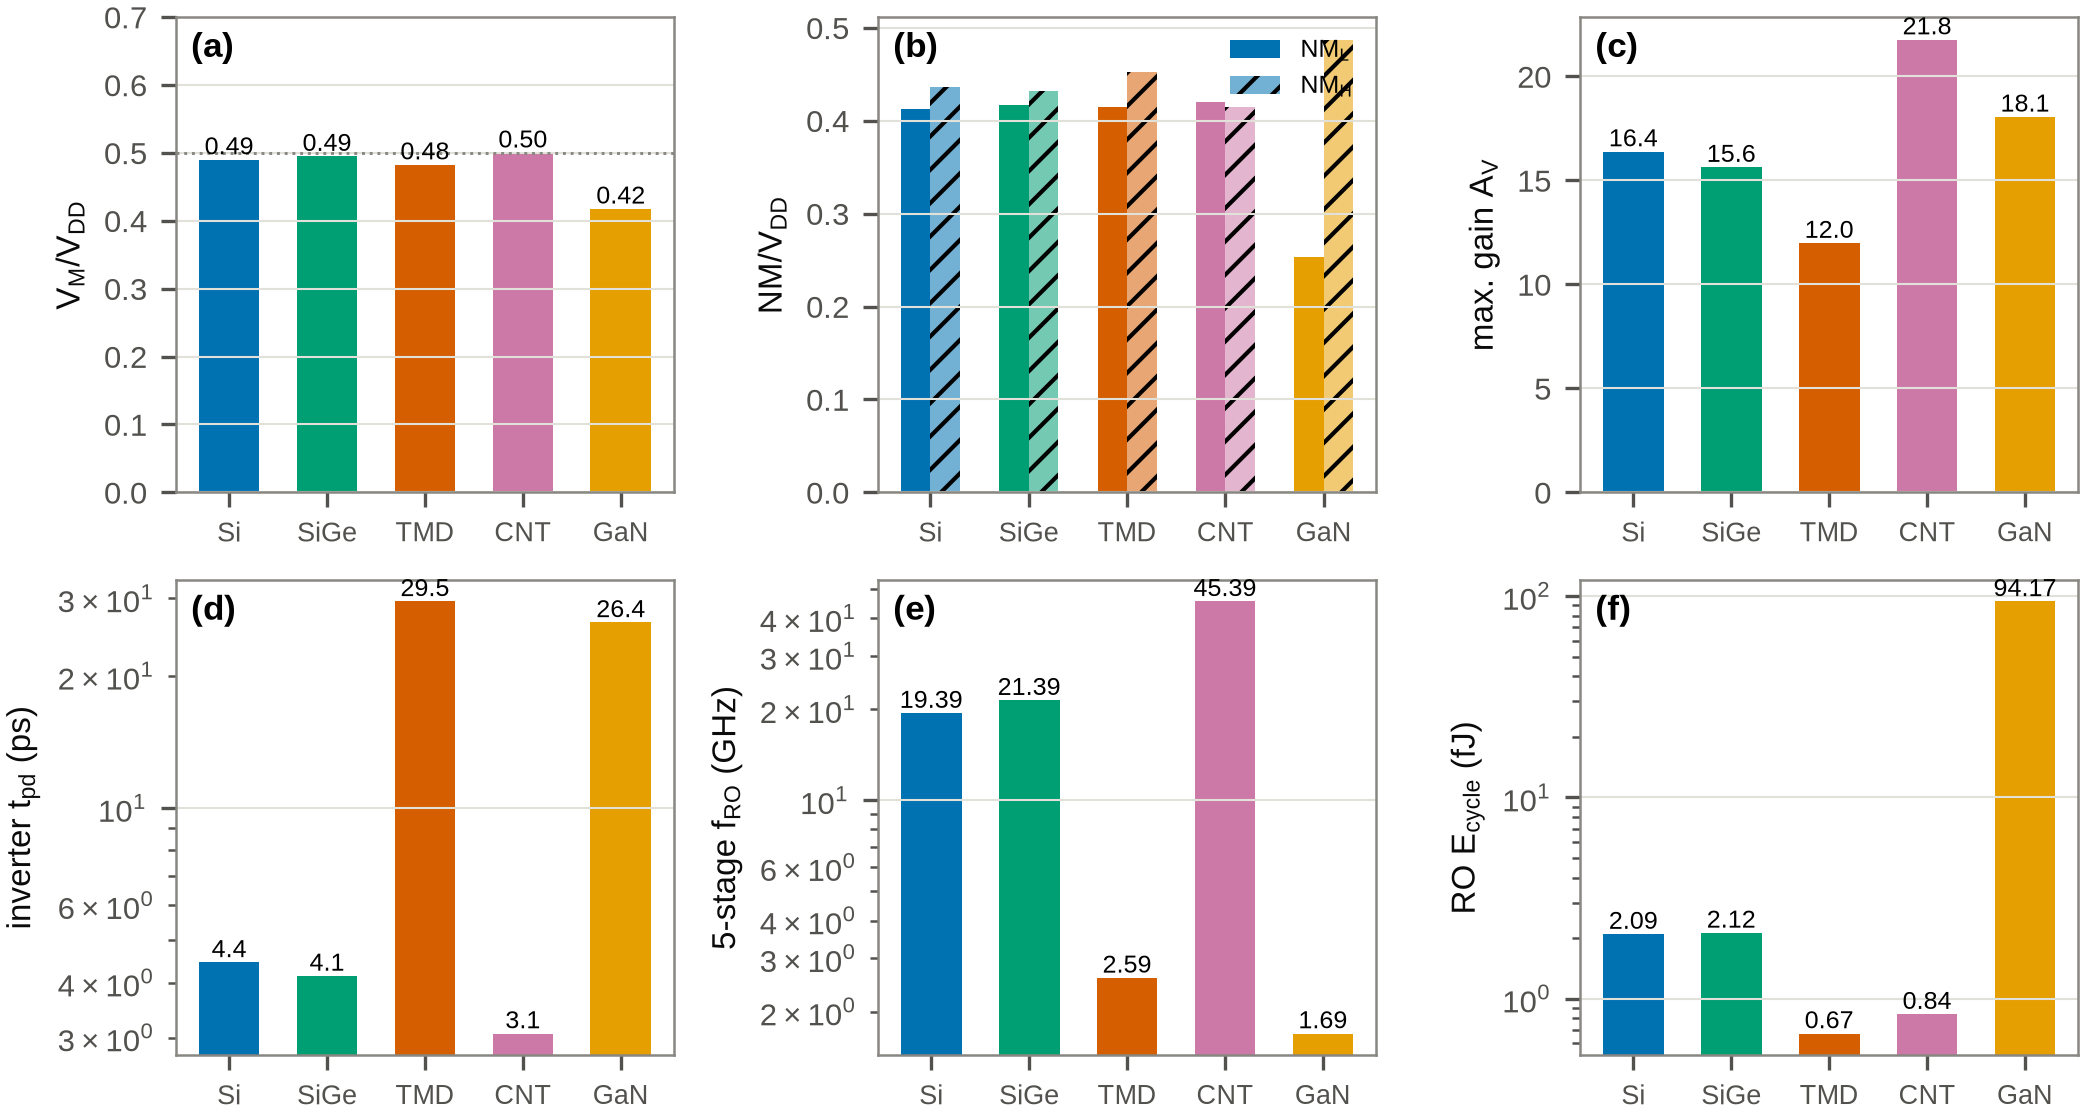
\includegraphics[width=\columnwidth]{fig06_inverter_ro_fom.png}
\caption{Nominal figures of merit: (a) $V_M/V_{DD}$, (b) noise margins, (c) maximum gain, (d) inverter delay, (e) 5-stage RO frequency, (f) energy per RO cycle.}
\label{fig:fom}
\end{figure}
\begin{figure}[!t]
\centering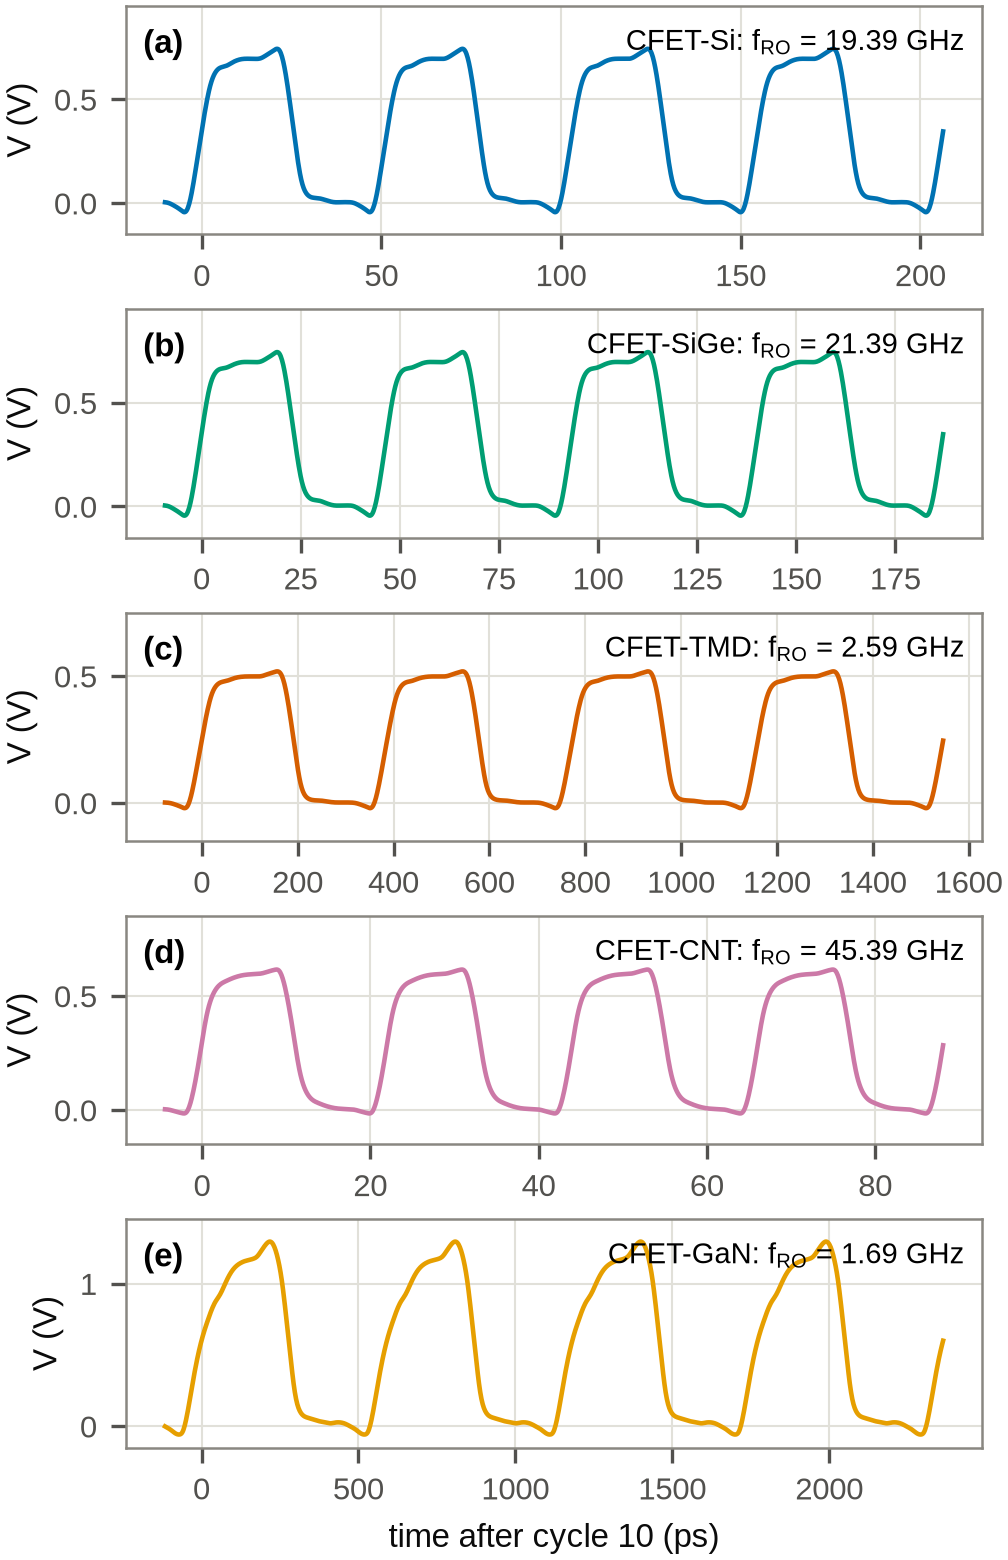
\includegraphics[width=\columnwidth]{fig07_ro_waveforms.png}
\caption{5-stage RO waveforms $V(n_3)$ for the five platforms, four cycles after cycle 10 (the measurement window).}
\label{fig:waves}
\end{figure}
\begin{table*}[!t]
\caption{Nominal inverter and 5-stage RO figures of merit (27$^\circ$C).}
\label{tab:nominal}
\centering\scriptsize
\begin{tabular}{lrrrrrrrrrr}
\hline
Platform & $V_{DD}$ & $V_M/V_{DD}$ & $A_V$ & $NM_L/V_{DD}$ & $NM_H/V_{DD}$ & $t_{pd}^{inv}$ & $f_{RO5}$ & $t_{pd}^{RO}$ & $P_{avg}$ & $E_{cycle}$ \\
 & (V) & & & & & (ps) & (GHz) & (ps) & ($\mu$W) & (fJ) \\
\hline
CFET-Si & 0.7 & 0.490 & 16.4 & 0.41 & 0.44 & 4.45 & 19.39 & 5.16 & 40.59 & 2.09 \\
CFET-SiGe & 0.7 & 0.495 & 15.6 & 0.42 & 0.43 & 4.14 & 21.39 & 4.68 & 45.40 & 2.12 \\
CFET-TMD & 0.5 & 0.482 & 12.0 & 0.41 & 0.45 & 29.51 & 2.59 & 38.68 & 1.74 & 0.67 \\
CFET-CNT & 0.6 & 0.500 & 21.8 & 0.42 & 0.41 & 3.06 & 45.39 & 2.20 & 38.01 & 0.84 \\
CFET-GaN & 1.2 & 0.418 & 18.1 & 0.25 & 0.49 & 26.43 & 1.69 & 59.06 & 159.43 & 94.17 \\
\hline
\end{tabular}

\end{table*}
Table~\ref{tab:nominal} and Figs.~\ref{fig:vtc}--\ref{fig:waves} give the nominal results. All five inverters are functional with $V_M/V_{DD}$ between \vmgan\ and \vmsi, gains between \gaintmd\ and \gaincnt\ and both noise margins above $0.28V_{DD}$; the SiGe p-FET moves $V_M$ of the SiGe cell closer to $V_{DD}/2$ than the Si cell (\vmsige\ vs. \vmsi) and shortens the low-to-high transition. The 5-stage RO frequencies are \frosi, \frosige, \frotmd, \frocnt\ and \frogan~GHz for Si, SiGe, TMD, CNT and GaN. Stage delays extracted from the 5-, 7- and 9-stage ROs agree within 1\%, which confirms the $1/(2Nf_{RO})$ extraction, while $E_{cycle}$ scales with $N$ as expected. The CNT platform is the fastest (quasi-ballistic injection, small gate charge) and has the second-lowest energy per cycle (\ecyccnt~fJ); the TMD platform is $7\times$ slower than Si at 0.5~V because of its 0.5--0.8~k$\Omega\cdot\mu$m contacts but has the lowest energy per cycle (\ecyctmd~fJ); the GaN platform is limited by the projected p-GaN device (hole mobility 20~cm$^2$/Vs, 3$\times$ up-sized) to \frogan~GHz and \ecycgan~fJ at 1.2~V. In the nominal GaN RO the average dissipation per device is only tens of microwatts, so the steady-state self-heating is a few kelvin and changes $f_{RO}$ by $<0.1$\%; it becomes significant only in the $R_{th}$ and temperature study below.

\subsection{Unified $V_{DD}$ and temperature sweeps}
\begin{figure*}[!t]
\centering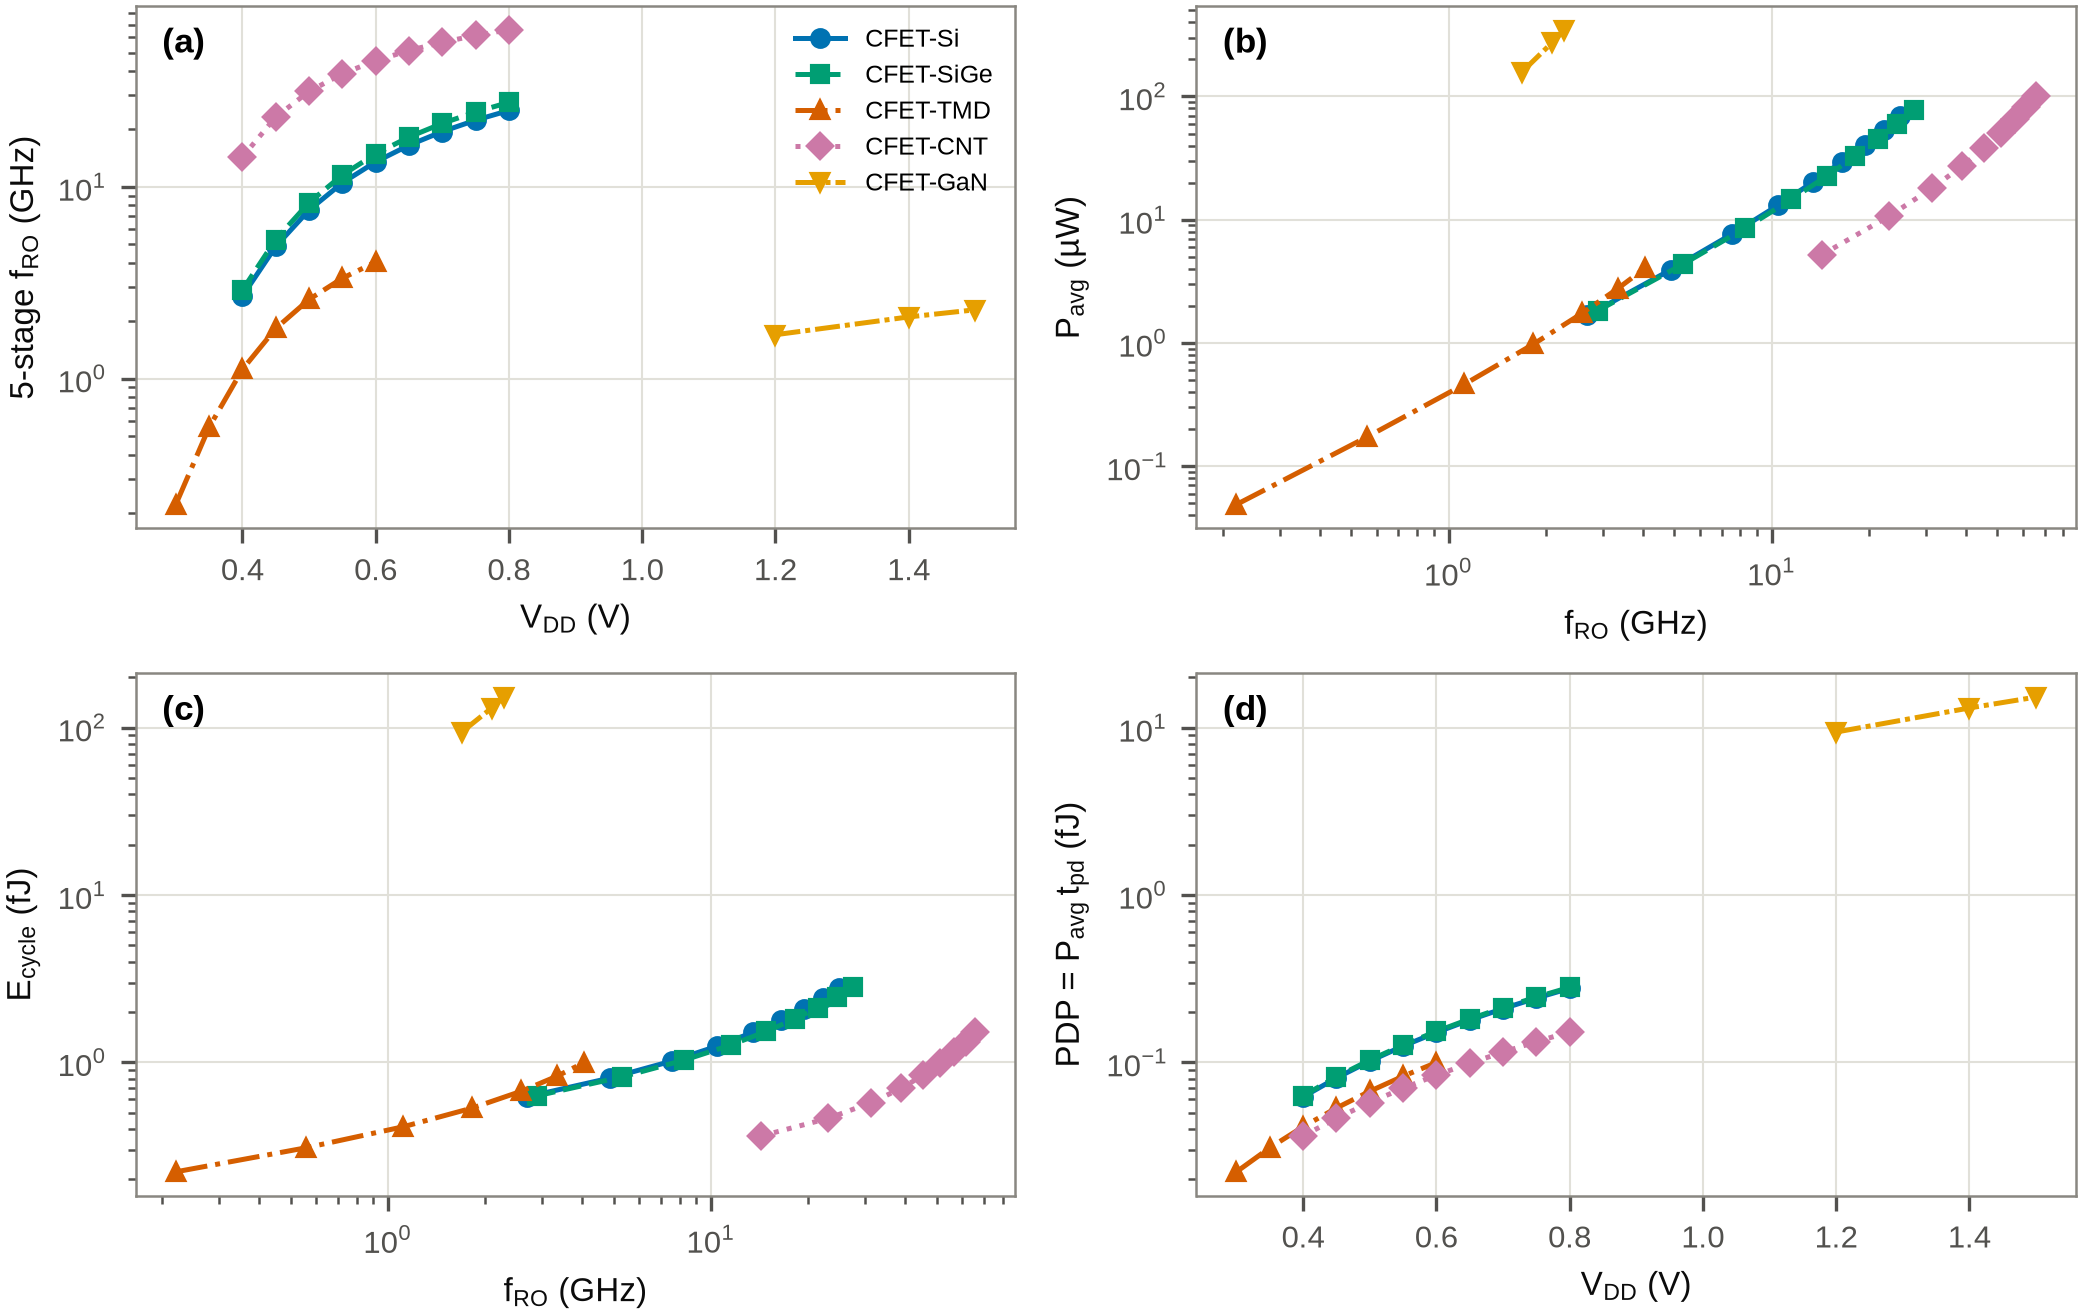
\includegraphics[width=\textwidth]{fig08_vdd_sweep.png}
\caption{Unified $V_{DD}$ sweeps of the 5-stage ROs: (a) $f_{RO}$ vs. $V_{DD}$, (b) power vs. frequency, (c) energy per cycle vs. frequency, (d) PDP vs. $V_{DD}$.}
\label{fig:vdd}
\end{figure*}
\begin{figure*}[!t]
\centering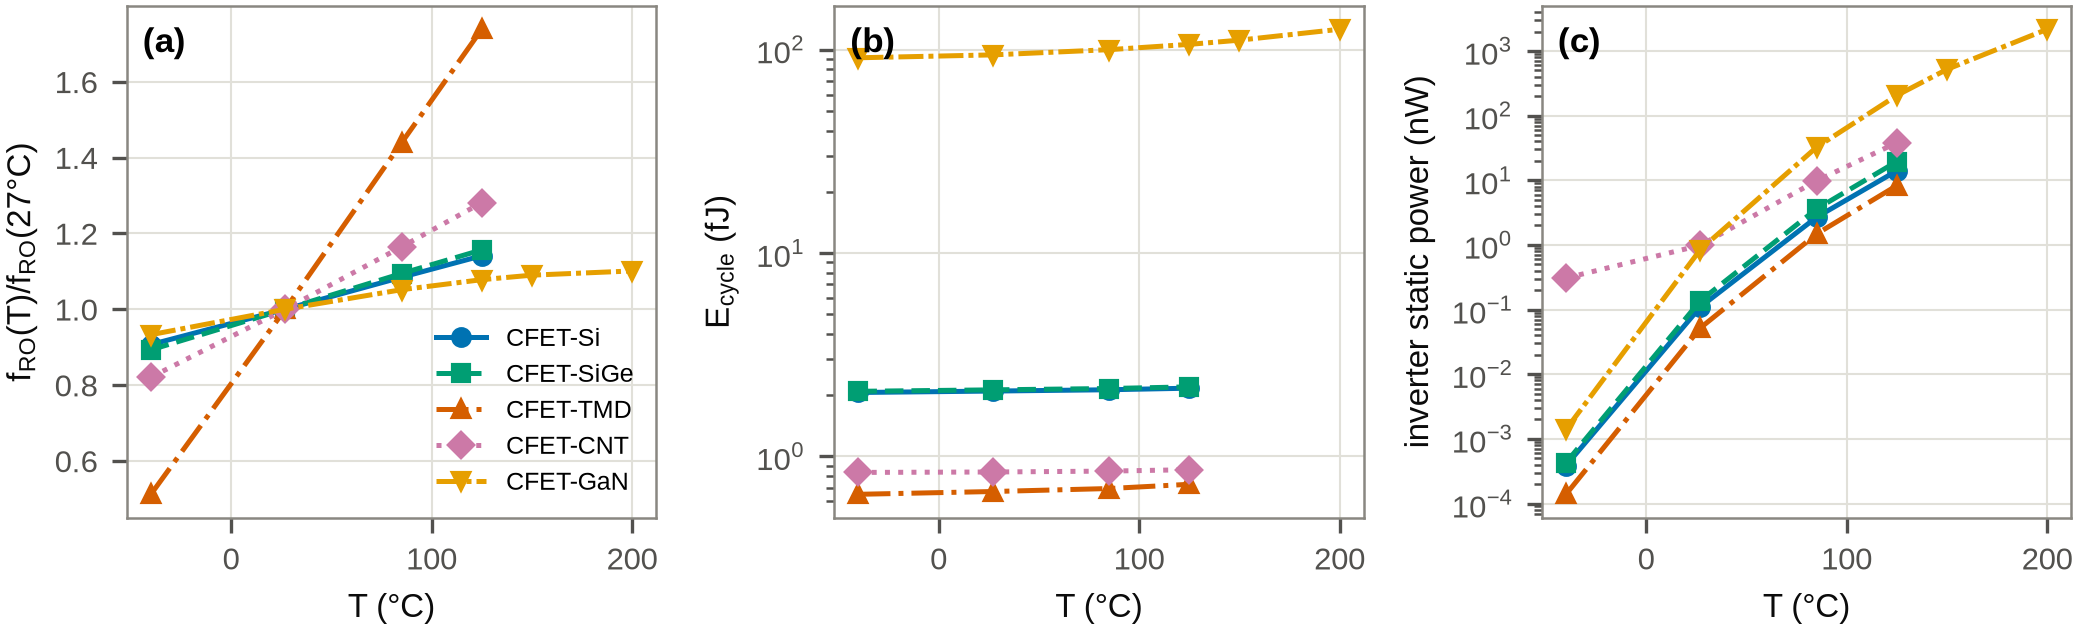
\includegraphics[width=\textwidth]{fig09_temperature.png}
\caption{Temperature sweeps at nominal $V_{DD}$ ($-40$ to 125$^\circ$C, GaN to 200$^\circ$C): (a) normalised $f_{RO}$, (b) energy per cycle, (c) inverter static power.}
\label{fig:temp}
\end{figure*}
Fig.~\ref{fig:vdd} compares the platforms on common axes. %%SWEEPTEXT
Fig.~\ref{fig:temp} shows the temperature behaviour. %%TEMPTEXT

\subsection{Material-specific sensitivity}
\begin{figure*}[!t]
\centering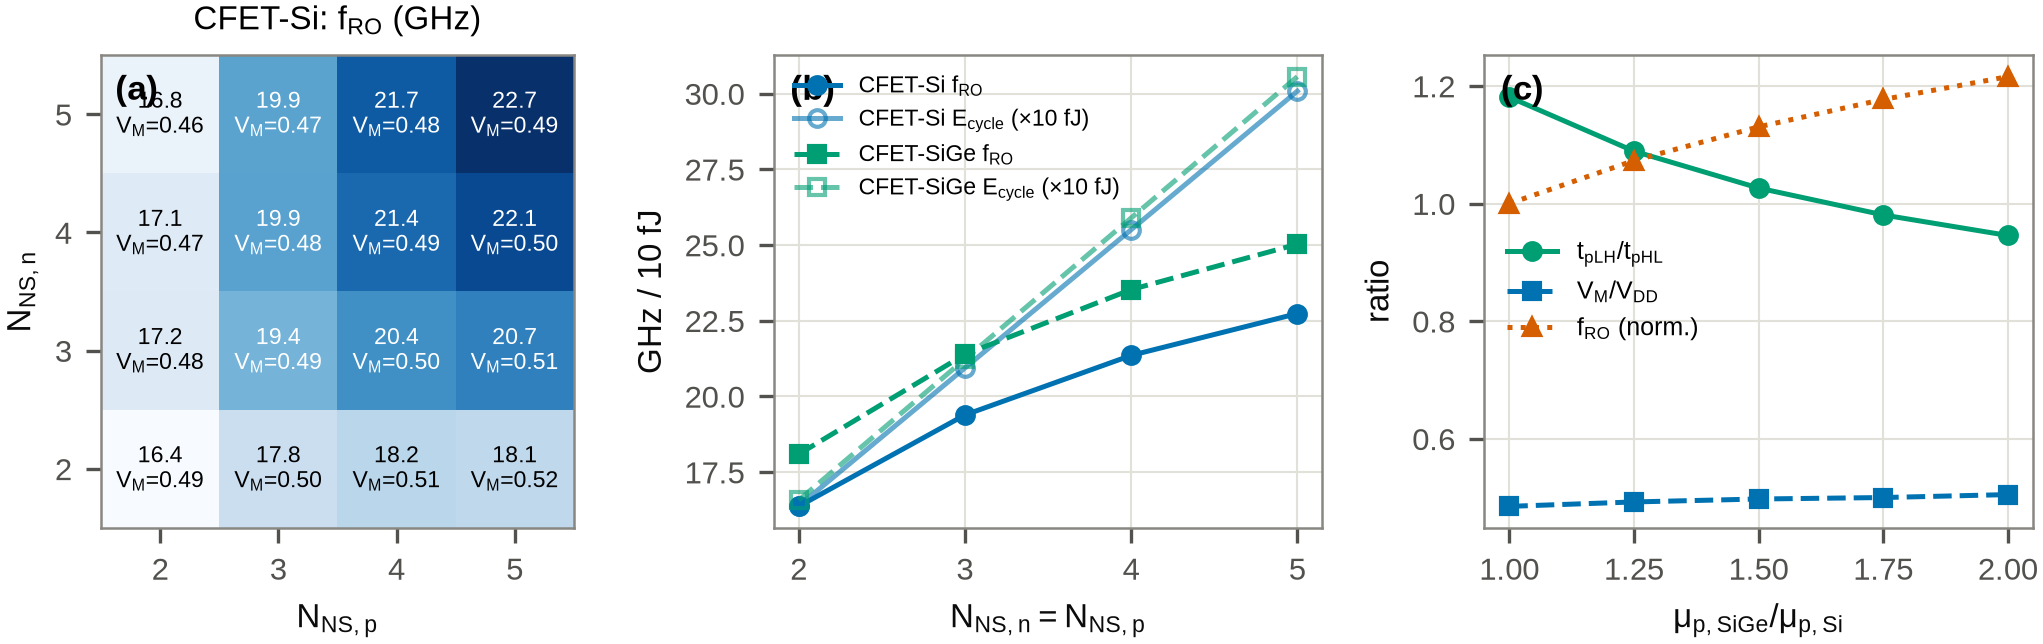
\includegraphics[width=\textwidth]{fig10_si_sige_sensitivity.png}
\caption{Si/SiGe study: 5-stage $f_{RO}$ and $V_M/V_{DD}$ vs. the number of nanosheets in the n- and p-tier for (a) CFET-Si and (b) CFET-SiGe; (c) effect of the SiGe/Si hole-mobility ratio on the rise/fall delay mismatch, $V_M$ and $f_{RO}$.}
\label{fig:sisige}
\end{figure*}
\begin{figure*}[!t]
\centering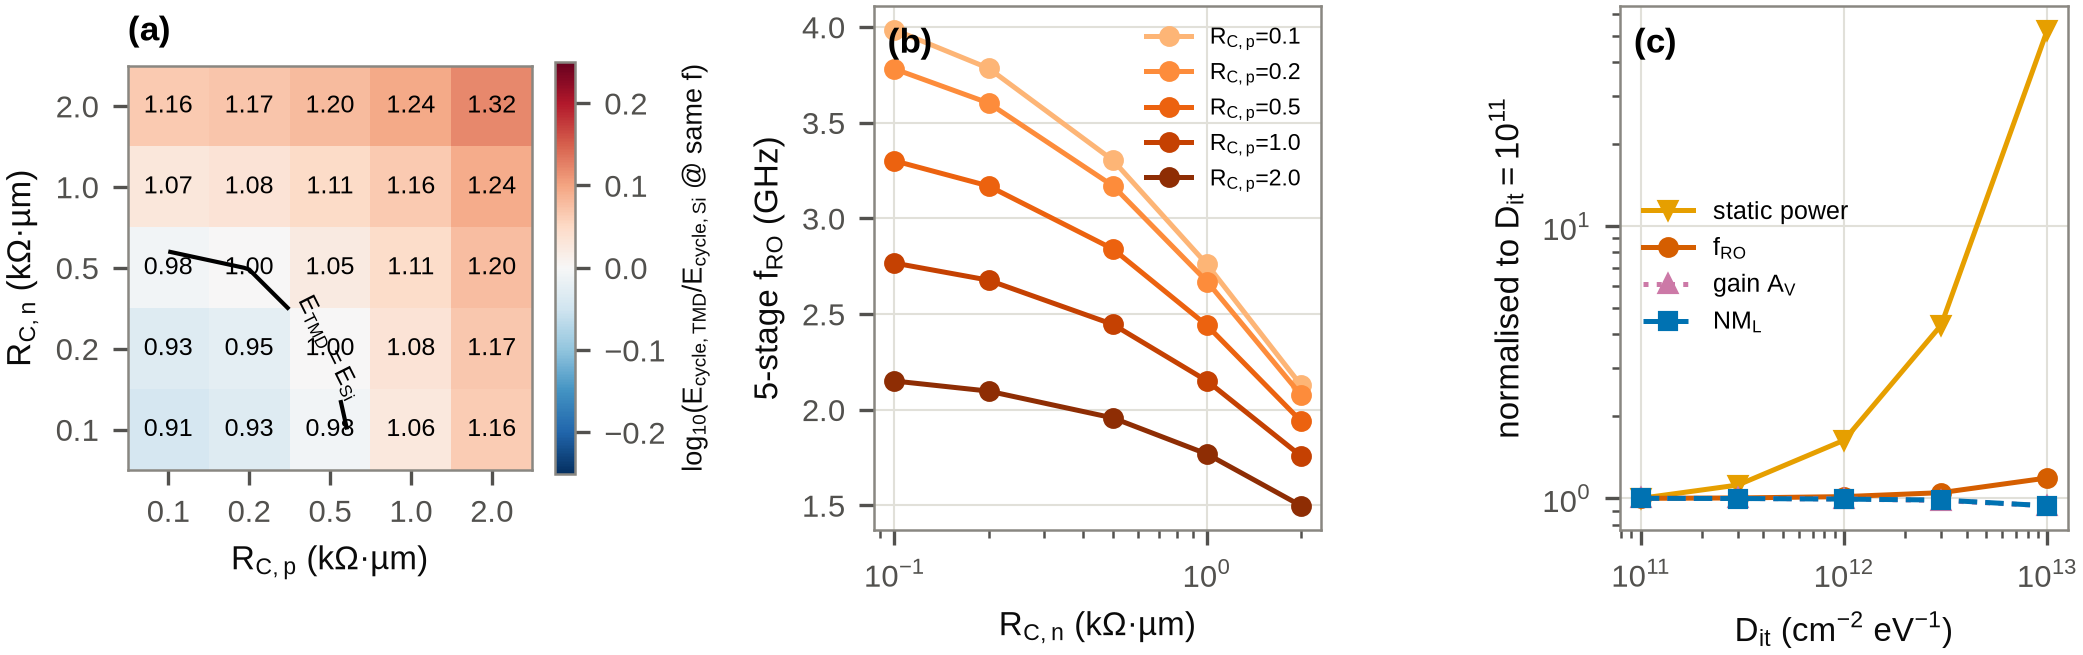
\includegraphics[width=\textwidth]{fig11_tmd_contact_crossover.png}
\caption{TMD study: (a) iso-frequency energy-per-cycle ratio $E_{TMD}/E_{Si}$ vs. the n- and p-contact resistance (the Si energy is interpolated at the TMD frequency from the Si $V_{DD}$ sweep extended to 0.3~V); (b) $f_{RO}$ vs. $R_{C,n}$; (c) effect of the interface trap density.}
\label{fig:tmd}
\end{figure*}
\begin{figure*}[!t]
\centering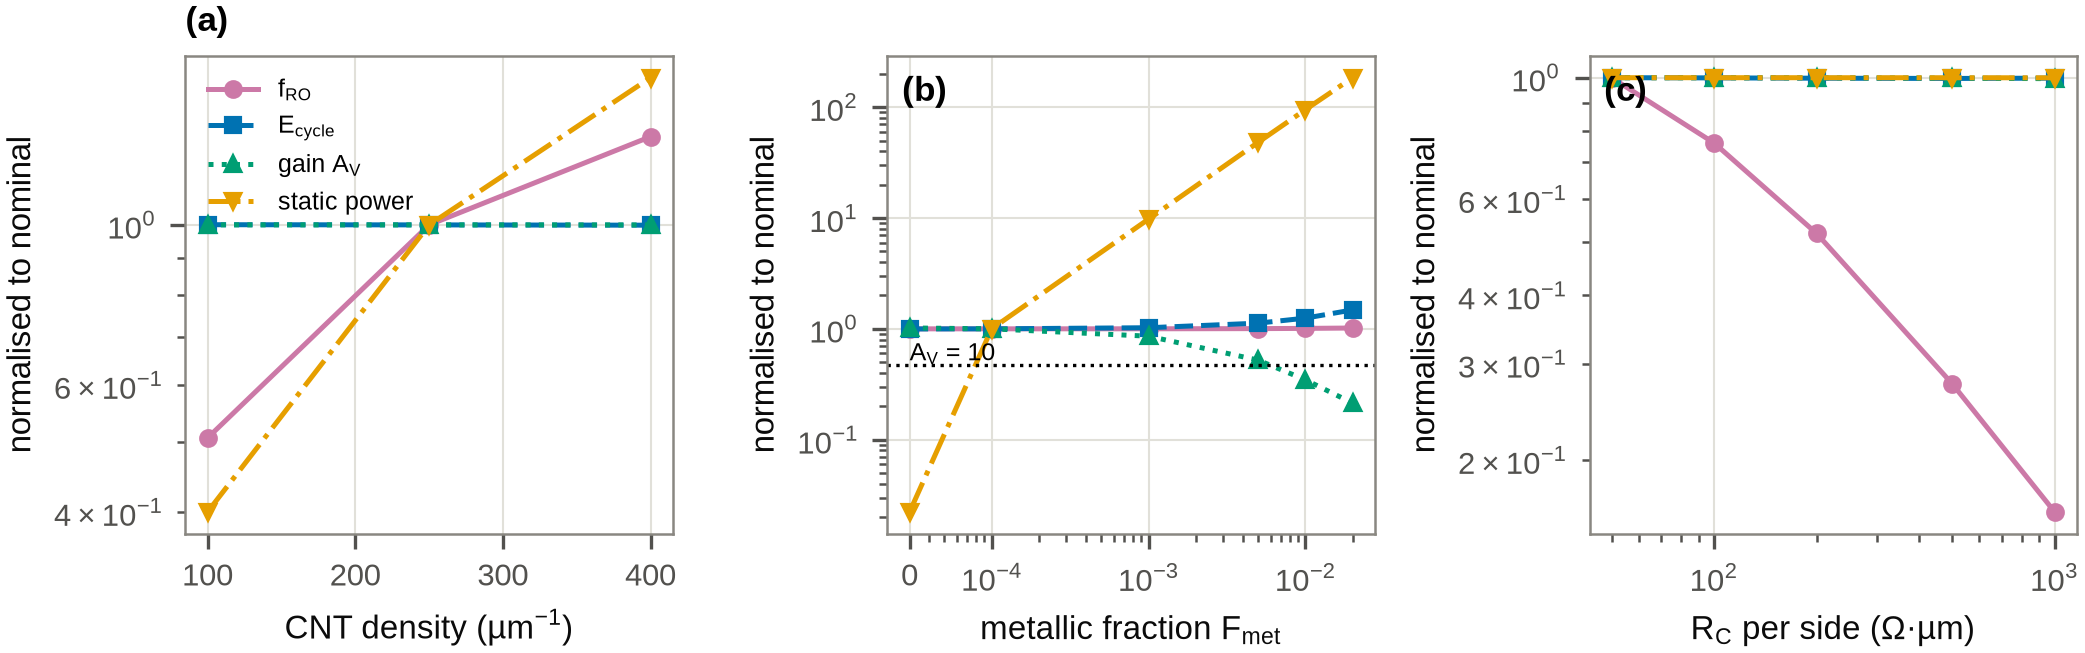
\includegraphics[width=\textwidth]{fig12_cnt_sensitivity.png}
\caption{CNT study: normalised $f_{RO}$ and PDP (left axes) and inverter static power (right axes) vs. (a) tube density, (b) metallic-tube fraction, (c) contact resistance.}
\label{fig:cnt}
\end{figure*}
\begin{figure*}[!t]
\centering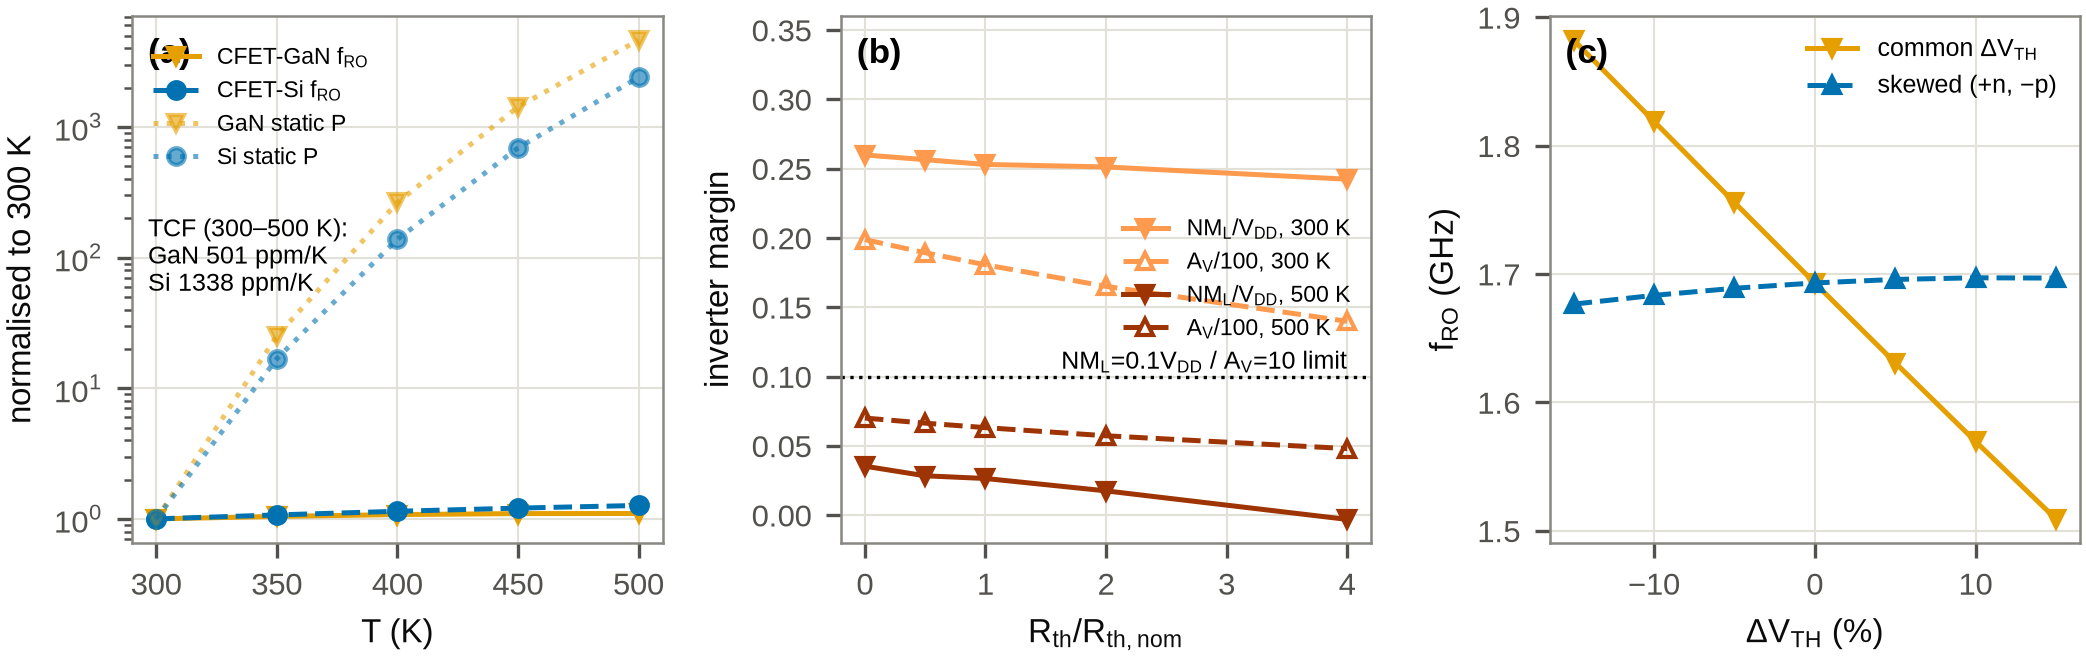
\includegraphics[width=\textwidth]{fig13_gan_thermal.png}
\caption{GaN study: (a) $f_{RO}$ and static power of CFET-GaN and CFET-Si from 300 to 500~K; (b) self-heating delay penalty vs. thermal resistance at three temperatures; (c) $f_{RO}$ vs. common and skewed threshold-voltage shifts.}
\label{fig:gan}
\end{figure*}
\subsubsection{Si and SiGe} %%SITEXT
\subsubsection{MoS$_2$/WSe$_2$} %%TMDTEXT
\subsubsection{CNT} %%CNTTEXT
\subsubsection{GaN} %%GANTEXT

\subsection{Monte Carlo and yield}
\begin{figure*}[!t]
\centering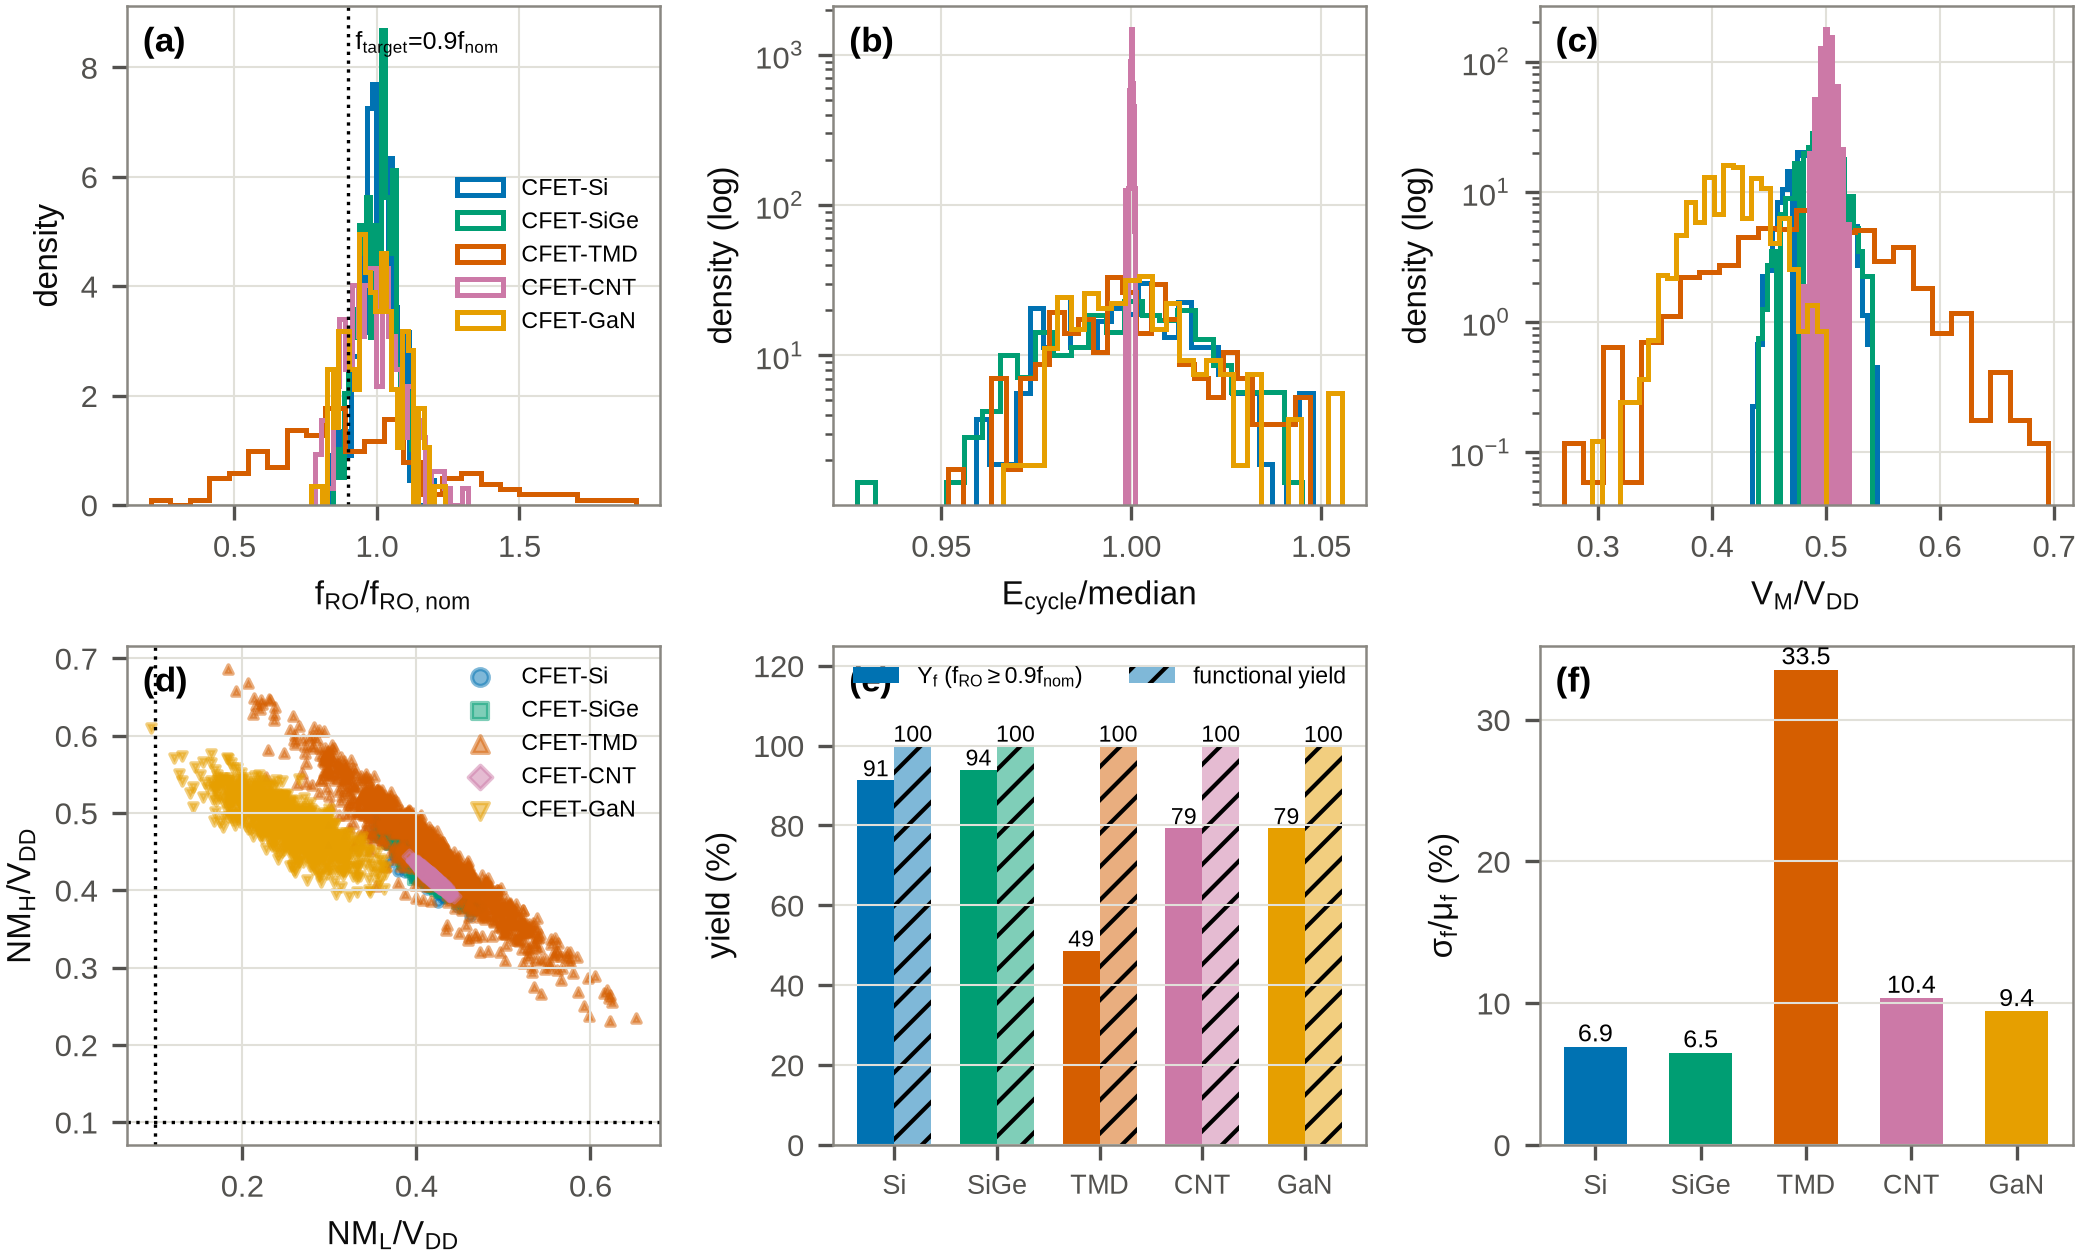
\includegraphics[width=\textwidth]{fig14_montecarlo.png}
\caption{Monte Carlo (200 RO samples and 1000 inverter samples per platform): (a) $f_{RO}$ normalised to nominal, (b) energy per cycle normalised to its median, (c) $V_M/V_{DD}$, (d) noise-margin scatter with the $0.1V_{DD}$ functional limits, (e) frequency yield $Y_f$ and functional yield, (f) relative frequency spread.}
\label{fig:mc}
\end{figure*}
\begin{table}[!t]
\caption{Monte Carlo summary and yield (criteria: $f_{RO}\geq0.9f_{RO,nom}$; $NM_{L,H}>0.1V_{DD}$ and $A_V>10$).}
\label{tab:mc}
\centering\scriptsize
\setlength{\tabcolsep}{3pt}\begin{tabular}{@{}lrrrrrrr@{}}
\hline
Platform & $N_{RO}$ & $\bar f_{RO}$ & $\sigma_f/\bar f$ & $Y_f$ & $\bar E_{cycle}$ & $N_{inv}$ & $Y_{func}$ \\
 & & (GHz) & (\%) & (\%) & (fJ) & & (\%) \\
\hline
CFET-Si & 150 & 19.35 & 6.9 & 91.3 & 2.10 & 1000 & 100.0 \\
CFET-SiGe & 150 & 21.43 & 6.5 & 94.0 & 2.12 & 1000 & 100.0 \\
CFET-TMD & 150 & 2.42 & 33.5 & 48.7 & 0.67 & 1000 & 100.0 \\
CFET-CNT & 150 & 44.87 & 10.4 & 79.3 & 0.84 & 1000 & 100.0 \\
CFET-GaN & 150 & 1.67 & 9.4 & 79.3 & 94.23 & 1000 & 99.9 \\
\hline
\end{tabular}

\end{table}
Monte Carlo was run only after the nominal VTCs, RO start-up and extraction had been verified for all platforms. The random variables are the physical model parameters listed in Section~III (Si: $V_{TH0}$ with $\sigma=20$~mV including work-function shift, $W_{NS}$ with $\sigma=1$~nm, $R_{SD}$ 10\%; SiGe adds 10\% on the p-mobility as a composition proxy; TMD: $R_C$ 30\% log-normal, $V_{TH0}$ 50~mV, mobility 20\%, $D_{it}$ 0.3~decades; CNT: density 15\%, metallic fraction log-normal around $10^{-6}$ with 0.5~decades, $R_C$ 30\%; GaN: $V_{TH0}$ 50~mV including trap shift, mobility 10\%, $R_{th}$ 20\%), drawn independently for the n- and p-device, with the same seeded generator for every platform. %%MCTEXT

\subsection{Conceptual layout}
\begin{figure*}[!t]
\centering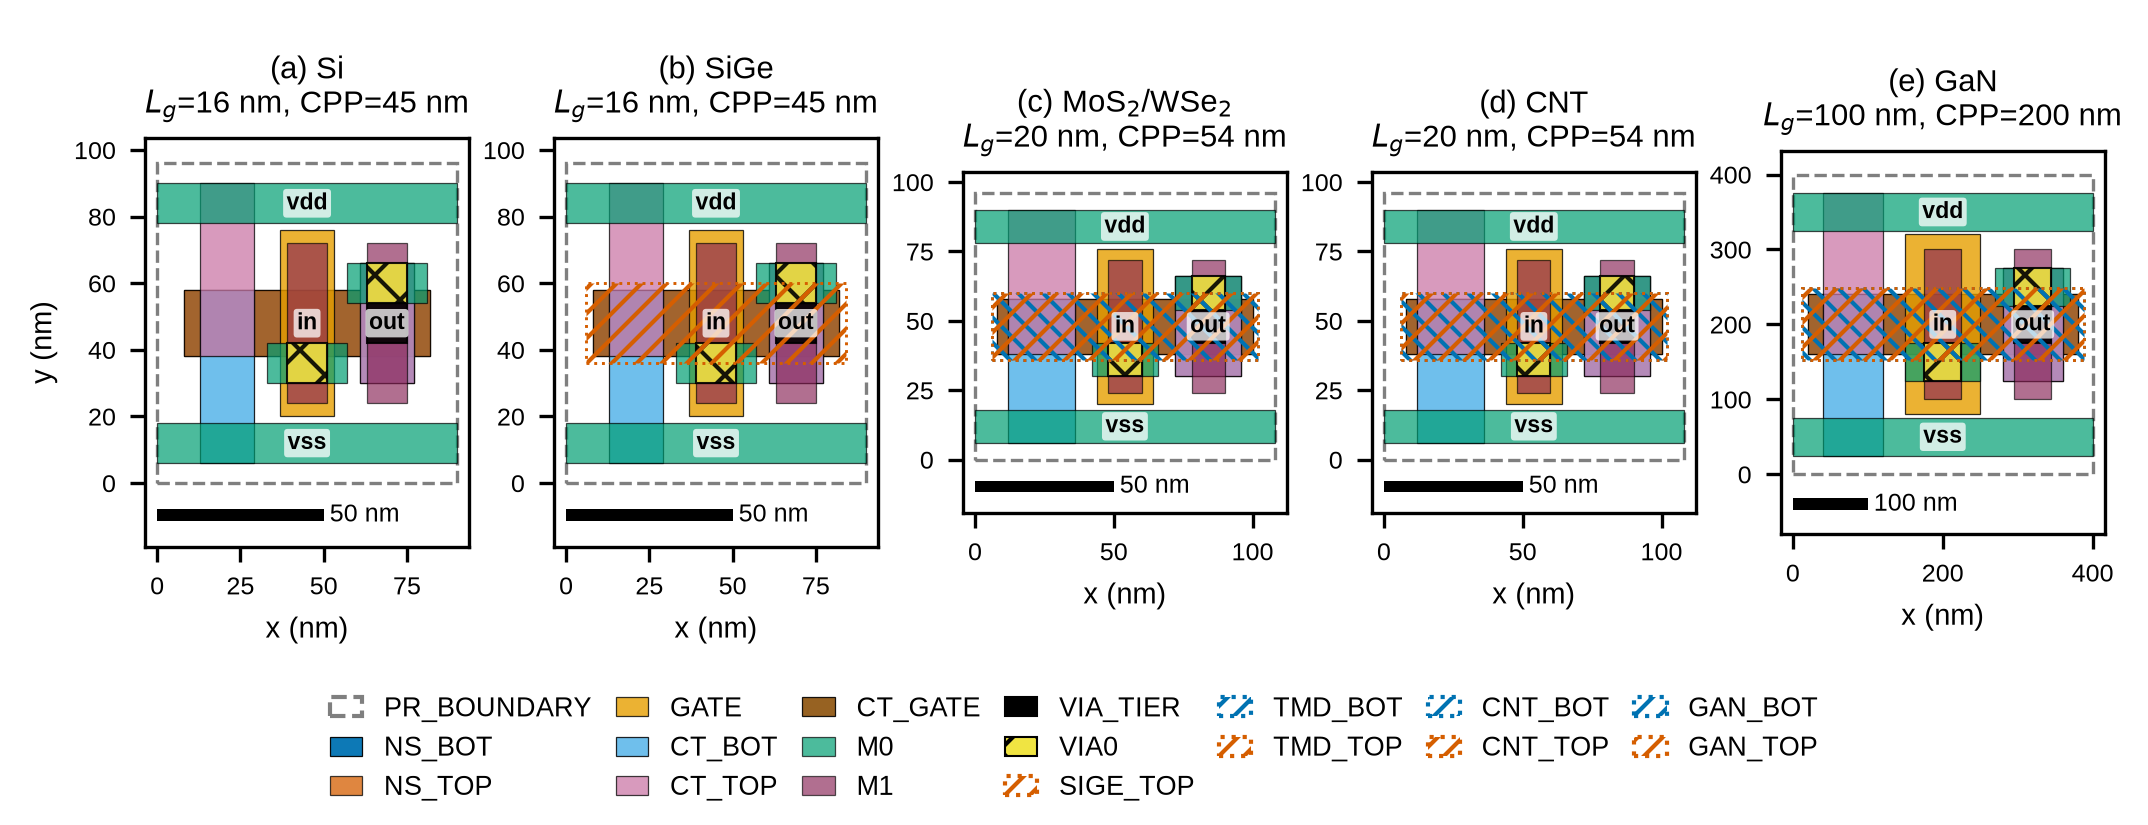
\includegraphics[width=\textwidth]{fig_layout_inverters.png}
\caption{Conceptual, DRC-clean GDSII layouts of the five CFET inverter cells (plan view; tiers drawn as separate layers): Si and SiGe at $L_g=16$~nm, CPP = 45~nm, 90$\times$96~nm cell; TMD and CNT projected at $L_g=20$~nm, CPP = 54~nm; GaN projected at $L_g=100$~nm, CPP = 200~nm.}
\label{fig:layout}
\end{figure*}
Fig.~\ref{fig:layout} shows conceptual layouts generated with a generic 3-nm-class CFET rule set (contacted gate pitch 45~nm, metal pitch 24~nm, 20-nm-wide nanosheets, four-track cell height because the p-tier folds over the n-tier). The bottom n-sheets, top p-sheets, common gate, tier contacts, inter-tier via joining the two drains and the M0 power rails are separate layers; a boolean DRC (minimum width and spacing per layer, gate-to-contact spacing, via enclosure) reports zero violations for the five inverters, the five 5-stage ROs and the top cell. The Si/SiGe inverter occupies $90\times96$~nm$^2$; the TMD/CNT projections $108\times96$~nm$^2$; the GaN projection $400\times400$~nm$^2$. These layouts annotate the gate length, sheet pitch, tier spacing and the location of $C_{stack}$; they are not tape-out-ready, which would require a real CFET PDK with DRC/LVS decks.

\section{Material-Selection Map}
\begin{figure}[!t]
\centering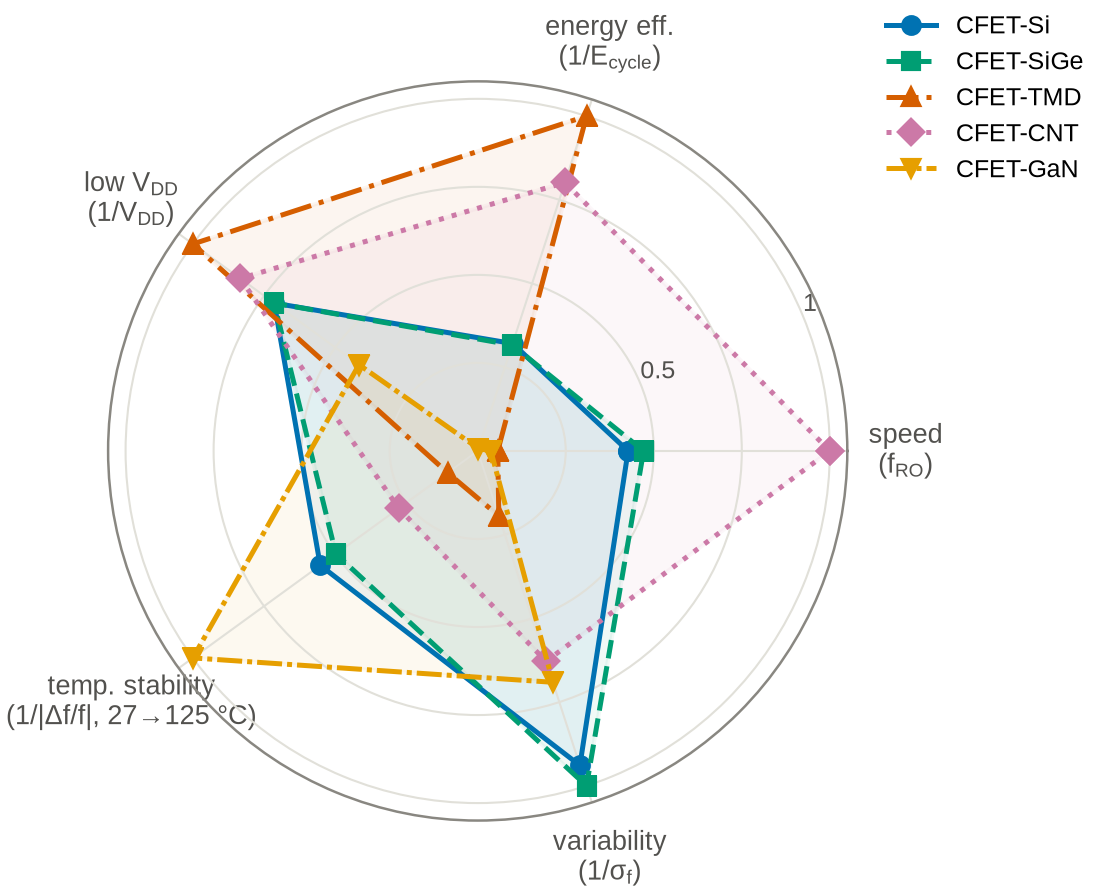
\includegraphics[width=0.9\columnwidth]{fig15_selection_chart.png}
\caption{Material-selection chart: speed, energy efficiency, low-$V_{DD}$ capability, temperature tolerance ($f_{125^\circ C}/f_{27^\circ C}$) and variability ($1/\sigma_f$), each normalised to the best platform.}
\label{fig:selection}
\end{figure}
Fig.~\ref{fig:selection} condenses the results. %%SELTEXT
\begin{table}[!t]
\caption{Selection map derived from the simulations.}
\label{tab:selection}
\centering\footnotesize
\begin{tabular}{p{0.46\columnwidth}p{0.46\columnwidth}}
\hline
Design need & Preferred CFET family \\ \hline
Highest maturity / main logic baseline & CFET-Si \\
Better p/n balance with Si-compatible processing & CFET-SiGe \\
Lowest $V_{DD}$, leakage-sensitive logic & CFET-TMD, if $R_C$ is below the crossover value (Fig.~\ref{fig:tmd}) \\
Highest performance post-Si research & CFET-CNT, if purity and density are controlled (Fig.~\ref{fig:cnt}) \\
High-temperature / integrated power-control logic & CFET-GaN (projected p-GaN) \\ \hline
\end{tabular}
\end{table}

\section{Limitations}
The reference data are literature-anchored reconstructions, not measurements; the MAPE values quantify the model's ability to follow an independent formulation, not agreement with hardware, and must be re-established with measured or TCAD curves before the models are used for a specific technology. The p-GaN device is a projection. The TMD block omits Schottky-barrier bias dependence of the contacts and the CNT block uses a single transmission parameter; the charge model uses a symmetric end-point partition rather than a full Ward--Dutton partition; CFET parasitics are lumped. The sensitivity and Monte Carlo trends, which are the main results, are driven by the physical parameters of the model and are therefore expected to be robust to these simplifications, but the absolute numbers should be read as platform-level projections.

\section{Conclusion}
A single compact-model core with four material blocks, implemented once in Verilog-A for Spectre/ADE and mirrored in ngspice, allows Si, SiGe, MoS$_2$/WSe$_2$, CNT and GaN CFET logic to be calibrated, simulated and compared with one flow and one set of measurement definitions. The flow reproduces a 5-stage RO at \frosi~GHz and \ecycsi~fJ/cycle for the Si baseline and yields a material-selection map: SiGe for p/n balance, TMD for the lowest energy at low $V_{DD}$ provided the contact resistance stays below the crossover value, CNT for the highest speed provided the metallic-tube fraction stays below $10^{-3}$, and GaN for high-temperature operation at an energy penalty set by the p-channel device. All models, scripts, layouts and results are released for reuse.

\balance
\bibliographystyle{IEEEtran}
\bibliography{refs}
\end{document}
